\documentclass[12pt, letterpaper, oneside, openany, spanish]{book} % book for the frontmatter and mainmatter

\pagestyle{myheadings} % para solo tener los numeros en el tope

\linespread{1.3} % Entre lineas de 1,5. Lo se, es raro

\setlength{\parskip}{10pt} % Doble espacio entre parrafos !!!!! Medir esto con un word

\title{Libro de pasantía Abril-Septiembre 2017}
\author{José Ricardo Pascarella Quijada} 
\date{\today}

\usepackage[left=3cm,top=2cm,right=2cm,bottom=2cm,bindingoffset=0.5cm]{geometry} 
\usepackage{xcolor,graphicx}
\usepackage[spanish]{babel} %Lenguaje Español
\usepackage[utf8]{inputenc} %Paquete para escribir acentos y otros símbolos directamente

\usepackage[acronym]{glossaries}
\loadglsentries[main]{abreviaturas}

\usepackage{biblatex}
\addbibresource{Bibliografia.bib}

\usepackage[toc,page]{appendix}

% for development %
\includeonly{Conclusiones}

% Tamanos de las fuentes
% 12pt option
% \tiny         	6pt
% \scriptsize     8pt
% \footnotesize   10pt
% \small         	11pt
% \normalsize     12pt
% \large         	14pt
% \Large         	17pt
% \LARGE         	20pt
% \huge         	25pt	
% \Huge         	25pt

% Capitulos en tamano 14 negrita, centrados con el nombre abajo y en mayusculas
\usepackage{titlesec}
\titleformat{\chapter}[display]   
{\normalfont\large\bfseries\centering}{\MakeUppercase{\chaptertitlename\ \thechapter}}{-10pt}{\bfseries\normalsize\MakeUppercase}
\titlespacing*{\chapter}{0pt}{0cm}{0cm}

% Secciones y subsecciones en tamano 12 y negrita
\titleformat*{\section}{\normalsize\bfseries}

\titleformat*{\subsection}{\normalsize\bfseries}

\newenvironment{dedication}
  {\vspace*{\stretch{1}}% some space at the top 
   \itshape             % the text is in italics
   \raggedleft          % flush to the right margin
  }
  {\par % end the paragraph
   \vspace{\stretch{3}} % space at bottom is three times that at the top
   \clearpage           % finish off the page
  }

\setcounter{secnumdepth}{3}
\setcounter{tocdepth}{3}


\begin{document}

	\frontmatter % Numeracion Romana
	 
		\begin{titlepage}
\begin{center}

\begin{figure}[h]
\begin{center}

\includegraphics{Logos/logoUSB.png}
\end{center}
\end{figure}

\textsc{UNIVERSIDAD SIMÓN BOLÍVAR}\\
\textsc{DECANATO DE ESTUDIOS PROFESIONALES}\\
\textsc{COORDINACIÓN DE INGENIRÍA DE LA COMPUTACIÓN}\\[8em]

\textsc{\Large \textbf{EXTENSIÓN DE UN SISTEMA DE MANEJO DE APRENDIZAJE CON UN MÓDULO DE ENCUENTROS PRESENCIALES}}\\[4em]

\textsc{ \textbf{Por:} }\\
José Ricardo Pascarella Quijada\\[4em]

\textsc{ \textbf{INFORME DE PASANTÍA} }\\
Presentado ante la Ilustre Universidad Simón Bolívar\\
como requisito parcial para optar al título de \\
Ingeniero en Computación

\vspace*{\fill}

\textsc{ \textbf{Sartenejas, Septiembre de 2017} }
\end{center}
\end{titlepage}
		\thispagestyle{empty} % No number in the tittle page
\begin{center}

\begin{figure}[h]
\begin{center}

\includegraphics{Logos/logoUSB.png}
\end{center}
\end{figure}

\textsc{UNIVERSIDAD SIMÓN BOLÍVAR}\\
\textsc{DECANATO DE ESTUDIOS PROFESIONALES}\\
\textsc{COORDINACIÓN DE INGENIRÍA DE LA COMPUTACIÓN}\\[8em]

\textsc{\Large \textbf{EXTENSIÓN DE UN SISTEMA DE MANEJO DE APRENDIZAJE CON UN MÓDULO DE ENCUENTROS PRESENCIALES}}\\[4em]

\textsc{ \textbf{Por:} }\\
\textsc{José Ricardo Pascarella Quijada}

\textsc{ \textbf{Realizado con la asesoría de:} }\\
\textsc{Prof. Federico Flaviani }\\
\textsc{Ing. Christian Ament}\\[4em]

\textsc{ \textbf{INFORME DE PASANTÍA} }\\
\textsc{Presentado ante la Ilustre Universidad Simón Bolívar}\\
\textsc{como requisito parcial para optar al título de }\\
\textsc{Ingeniero en Computación}

\vspace*{\fill}

\textsc{ \textbf{Sartenejas, Septiembre de 2017} }
\end{center}


		% Para meter los graficos del acta escaneada
\mbox{}
\thispagestyle{empty}
\newpage

\mbox{}
\thispagestyle{empty}
\newpage

		\begin{center}
	
	\begin{figure}[h]
		\begin{center}
		
\includegraphics[width=0.1\textwidth]{logos/logoUSB.png}
		\end{center}
	\end{figure}

	\textsc{UNIVERSIDAD SIMÓN BOLÍVAR}\\[0.1pt]
	\textsc{DECANATO DE ESTUDIOS PROFESIONALES}\\
	\textsc{COORDINACIÓN DE INGENIERÍA DE LA COMPUTACIÓN}

	\textsc{\textbf{EXTENSIÓN DE UN SISTEMA DE GESTIÓN DE APRENDIZAJE CON UN MÓDULO DE ENCUENTROS PRESENCIALES}}

	Realizado por: José Ricardo Pascarella Quijada\\
	Con la asesoría de:	Prof. Federico Flaviani e Ing. Christian Ament

	\textsc{\textbf{RESUMEN}}

\end{center}

Este documento presenta detalladamente el proceso de desarrollo de una extensión para un \gls{SGA} que permite el soporte de encuentros presenciales o seminarios entre estudiantes e instructores. 

El módulo apoya a tres tipos de usuarios en la gestión de los encuentros. Los administradores, que crean los cursos y asignan los instructores. Los instructores que pueden administrar la asistencia y calificación; por último, los estudiantes que seleccionan cursos a los que asistir.

Para la realización de este módulo se usó la metodología de desarrollo de \emph{software} ágil e iterativo por fases \emph{scrum}. Para el desarrollo se utilizó el conjunto de soluciones informáticas \gls{WAMP}, que consiste en Windows como plataforma de sistema operativo, Apache para el servicio web, \gls{SQL} Server con gestor de bases de datos y el lenguaje multipropósito \gls{PHP}.

Se logró mediante este proyecto que el SGA base de la compañía contenga la nueva funcionalidad, que permite ser extendida y personalizada dependiendo de las necesidades de distintos clientes. Además, el módulo se implantó con éxito en la arquitectura de un cliente que previamente poseía el servicio de \gls{SGA}.

\textbf{Palabras clave}: \gls{SGA}, \gls{PHP}, desarrollo, seminario.






		% \chapter*{Dedicatoria}

A mi madre que me ha dedicado su vida

A mi padre que siempre me apoya y nunca deja de aconsejarme

A mi tía Evelin que me tomó en serio desde los 8 años, mucho antes de que yo lo hiciera 

Los amo. 
		% \chapter*{Agradecimientos}

A mis padres y mi tía Evelin, por ser siempre un impulso y un apoyo que me ha permitido llegar a lugares a los que nunca me hubiese imaginado, gracias a ustedes puedo decir que nunca me ha faltado nada, sobre todo amor.

Al resto de la familia por propiciar el mejor ambiente para mi desarrollo, en ustedes constantemente encuentro ejemplos a seguir, consejos, cariño y una inmesa responsabilidad de recordar de donde vengo con orgullo compartir los valores que de ustedes y con ustedes aprendí. 

A Clara Cangiano, te separo aqui de la familia, pero solo para que sepas que a ella perteneces. Gracias por compartir toda tu vida conmigo, de ti he aprendido mucho. El amor sin una cesta llena haz como que no lo has visto. Siempre mantuviste la cesta llena. No creas que olvidaré la promesa que te hice.

A mis amigos mas cercanos, cada uno con un aporte muy especial: Guillermo Hernández, con el que siempre fue bueno competir, pero al mismo tiempo me recordó ser humilde, no te quedes atras. Luis Colorado, una de esas personas que a veces no te crees que existen, su entrega y positividad es única. Rafael Delgado, siempre estas allí viejo, nos veremos pronto. Mailyn Guevara por lo fácil que es compartir todo contigo y Fabiana Abdallah, gracias a tí valoro la sinceridad y entiendo que se puede conseguir.

A la gente del Laboratorio Docente de Aulas Computarizadas (MAC). No solo por ser mi casa en Caracas, si no por hacer de esa casa un hogar. Compartir con ustedes cada día fue una experiencia única de aprendizaje y superación sobre la computación y la vida. La mejor decisión que he tomado es hacer esa admisión.

A todas las demás personas que hacen vida en la Universidad Simón Bolívar, junto y gracias a ustedes no solo me formé como ingeniero, dadas las circunstancias, aprendí que hay que luchar, que la vida no es fácil, junto a ustedes estuve luchando en todos los frentes codo a codo y el que se roza con diamantes de alguna forma se pule.

Luis Colorado y Andres Navarro, gracias por hacer los últimos pasos no solo amenos, sino posibles, que viva el tridente.

		\tableofcontents % Indice
		\listoffigures
		\printglossary[type=\acronymtype]

	\mainmatter % Comienzo de numeracion arabica

		\chapter*{Introducción}
\thispagestyle{empty} % Quitar el número
\addcontentsline{toc}{chapter}{Introducción} \markboth{INTRODUCCIÓN}{}
El presente documento describe el proceso de desarrollo del módulo de encuentros presenciales para un SAG (Sistema de Gestión de Aprendizaje) para Fischer Knoblauch \& Co (FKC) como proyecto de pasantías realizado por su autor.

\section*{Antecedentes}
\addcontentsline{toc}{section}{Antecedentes}
El SGA básico de FKC es un producto que soporta las funciones basicas de cualquier sistema de gestión aprendizaje simple. Como lo son: manejo de usuarios y contenidos; segimiento del proceso de aprendizaje, evaluaciones y herramientas de comunicación como foros y mensajes privados. Este sistema es personalizado e instalado generalmente en la infraestructura del cliente según sus necesidades.

\section*{Justificación e importancia}
\addcontentsline{toc}{section}{Justificación e importancia}
Entre las funciones convencionales de los SGA actuales se encuentra el manejo de encuentros presenciales, funcionalidad considerada como necesaria por actuales y potenciales clientes. Siendo estos encuentros de importancia crítica para el flujo del conocimiento de mediana a alta complejidad que no puede ser expresado facilmente por medio de cursos en linea. Por lo tanto, es de interés para la compañia poseer esta funcionalidad en su sistema.


\section*{Planteamiento del problema}
\addcontentsline{toc}{section}{Planteamiento del problema}
Se identificó la necesidad de extender el sistema de FKC con un módulo que le permita a sus clientes gestionar encuentros presenciales entre instructores y estudiantes. Al mismo tiempo este módulo debía adaptarse a la estructura de cursos y grupos previamente existente en el sistema trantando de incluir la menor complejidad posible para su futura extensión y personalización.

Para lograr esto, es necesario un profundo entendimiento del producto, con el fin de desarrollar un módulo que mantenga el mismo estilo tanto en la programacion, como en el funcionamiento y la interfaz. 


\section*{Objetivos}
\addcontentsline{toc}{section}{Objetivos}
A continuación, se exponen los objetivos generales y específicos que se busca alcanzar en este desarrollo con la finalidad de contextualizar al lector respecto al informe de este proyecto de pasantía.

\subsection*{Objetivo general}
\addcontentsline{toc}{subsection}{Objetivo general}
El objetivo general de este proyecto es desarrollar un módulo que permita extender el sistema de gestión de aprendizaje con un módulo que lo acerque a contener las funciones convencionales de los sistemas en la actualidad y que al mismo tiempo posea la flexibilidad de ser personalizado para las distintas necesidades de los clientes o hasta no ser incluido de no ser necesario.

\subsection*{Objetivos específicos}
\addcontentsline{toc}{subsection}{Objetivos específicos}
Extender la Base de Datos para el soporte del módulo.

Desarrollo de un módulo que permita el manejo de las locaciones donde se imparten los seminarios por parte del administrador.

Integrar el nuevo tipo de curso a las funcionalidades previas de administrador sobre otros tipos de cursos, como estadísticas y asignación a grupos.

Creación de un nuevo tipo de usuario, instructor, que tenga potestad sobre los seminarios.

Integrar el nuevo tipo de cursos en la interfaz del estudiante del sistema.

Integrar el módulo tanto en el sistema base de FKC como en uno de los clientes que poseen un versión personalizada del sistema.










		\chapter{Entorno Empresarial}
\thispagestyle{empty} % Quitar el número

En este capítulo se describe el entorno empresarial en el cual tuvo lugar el desarrollo del proyecto de pasantía, la empresa \gls{FKC} filial de Frankfurt.

\section{Fischer, Knoblauch \& Co.}

Es un proveedor de servicios multimedia especializado en el área de aprendizaje electrónico. Está presente en Frankfurt y Munich en Alemania así como en Basel, Suiza. Fundada en 1996 por Guy Fischer y Thomas Knoblauch.

Proveen consultoría en la integración y ampliación del aprendizaje electrónico a compañías de diversos sectores en Alemania y Bélgica. Se encargan de sugerir la elección de tecnologías, concepción del plan de aprendizaje, didácticas y metodología de la enseñanza, producción del contenido audiovisual, hasta la integración de la solución en el ambiente del cliente. 

Si una compañía requiere enseñar una cierta habilidad a sus empleados contacta a un proveedor de servicios de aprendizaje electrónico, \gls{FKC} los ayuda a integrar un plan aprendizaje a su empresa, que se ven materializados en entrenamientos basados en la web. 

\gls{FKC} también posee un Sistema de Gestión de Aprendizaje, la pieza de \emph{software} en la que el pasante trabajó, que es personalizable y permite la organización de estos entrenamientos creados por la empresa.

Además, \gls{FKC} haciendo uso de su departamento gráfico y programadores, también provee servicios de posicionamiento empresarial en la web, mediante la creación de páginas, logos y demás contenido multimedia que la compañía requiera. 

Sus programadores día a día se enfrentan con diversos retos informáticos en distintos lenguajes de programación. Estos pueden ser: migraciones de sistemas de bases de datos, internacionalización de sus aplicaciones que llegan a estar hasta en diez lenguajes distintos, diseño de soluciones multiplataforma y el manejo e instalación de \emph{frameworks} que faciliten la construcción de soluciones multimedia.

\section{Estructura organizacional}

En la figura \ref{fig:estructuraFKC} se muestra la estructura organizacional de \gls{FKC} Frankfurt:

\begin{figure}[h]
\begin{center}
	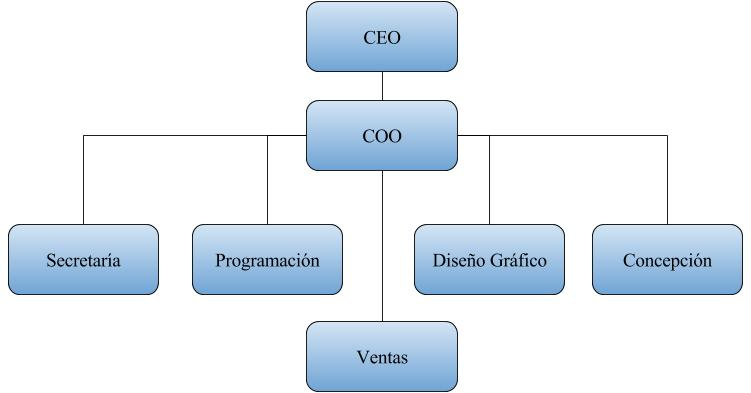
\includegraphics[width=\textwidth]{figuras/estructuraFKC.jpg}
	\caption{Estructura organizacional de \gls{FKC}.} \label{fig:estructuraFKC}
\end{center}
\end{figure}

\gls{FKC} Frankfurt es un equipo multidisciplinario donde es importante la comunicación entre los distintos \emph{stakeholders}. Los creadores de concepto se unen a los diseñadores y los programadores para plasmar fielmente los requerimientos del cliente y obtener como resultado una solución hecha a la medida.

A continuación una descripción breve de los cargos en el organigrama.

Director Ejecutivo es la persona de máxima autoridad, encargada de la gestión y dirección administrativa en la organización.

Director de Operanciones es el responsable del control de las actividades diarias de la corporación y de manejo de las operaciones. Reporta directamente al director ejecutivo.

Secretaría encargada de dar apoyo a los empleados de la empresa en cuanto a la gestión de papeleo y la comunicación de las actividades.

La cuadrilla de programación se encarga de materializar las peticiones que llegan de los demás departamentos mediante soluciones informáticas.

El grupo de diseño gráfico se encarga de generar el material multimedia junto con los integrantes del grupo de concepción y los clientes. 

El departamento de ventas se encarga del \emph{marketing} de los productos ofrecidos por \gls{FKC}.

\section{Cargo ocupado por el pasante} 

El pasante perteneció al grupo de programación que se muestra en la figura \ref{fig:estructuraFKC} donde formó parte de un equipo de 6 programadores.




		\chapter{Marco Teórico}
\thispagestyle{empty} % Quitar el número

En el presente capítulo es presentado y descrito el conjunto de conceptos, términos y pilares teóricos relevantes sobre el cuales se basó este proyecto.

\section{Conceptos básicos sobre el area de trabajo}

\subsection{E-learning o aprendizaje electrónico}

Se denomina aprendizaje electrónico (conocido también por el anglicismo \emph{e-learning}) a la educación a distancia completamente virtualizada a través de los nuevos canales electrónicos (las nuevas redes de comunicación, en especial Internet), utilizando para ello herramientas o aplicaciones de hipertexto (correo electrónico, páginas web, foros de discusión, mensajería instantánea, plataformas de formación -que aúnan varios de los anteriores ejemplos de aplicaciones-, etc.) como soporte de los procesos de enseñanza-aprendizaje.

Gracias a las nuevas tecnologías de la información y la comunicación (TIC), los estudiantes “en línea” pueden comunicarse y colaborar con sus compañeros “de clase” e instructores (profesores, tutores, mentores, etc.), de forma síncrona o asíncrona, sin limitaciones espacio-temporales. Es decir, se puede entender como una modalidad de aprendizaje dentro de la educación a distancia en la que se utilizan las redes de datos como medios (Internet, intranets, etc.), las herramientas o aplicaciones hipertextuales como soporte (por ejemplo, correo electrónico, web, chat, etc. ) y los contenidos y/o unidades de aprendizaje en línea como materiales formativos. Como ejemplo, simples imágenes, audio, video, documentos, llegando hasta complejas producciones multimedia.

Las ventajas que ofrece la formación en línea son las siguientes:

Eliminación de barreras espaciales y temporales (desde su propia casa, en el trabajo, en un viaje a través de dispositivos móviles, etc.). Supone una gran ventaja para discentes geográficamente dispersos o alejados.
Prácticas en entornos de simulación virtual, difíciles de conseguir en formación presencial, sin una gran inversión.
Enriquecimiento colectivo del proceso de aprendizaje sin límites geográficos.
Actualización constante de los contenidos (deducción lógica del punto anterior).
Reducción de costos (en la mayoría de los casos, a nivel metodológico y, siempre, en el aspecto logístico).


Es una alternativa de formación que no reemplaza necesariamente a los profesores y las clases presenciales, sino que es un espacio que desarrolla la autonomía del aprendiz.

\subsection{B-learning o aprendizaje híbrido}

En un concepto más relacionado con lo semipresencial, también está el llamado b-learning (blended learning). Esto significa que un curso dictado en este formato incluirá tanto clases presenciales como actividades de e-learning.

Este modelo de formación hace uso de las ventajas de la formación 100\% on-line y la formación presencial, combinándolas en un solo tipo de formación que agiliza la labor tanto del formador como del alumno. La enseñanza combinada o mezclada, a veces también denominada enseñanza híbrida se define como cursos o programas en los que el contenido online supone entre un 30\% y un 70\% del total del curso. En contraste, la enseñanza presencial incluye aquellos cursos en los que el contenido online oscila entre 0\% y 29\% del curso. Las ventajas que se suelen atribuir a esta modalidad de aprendizaje son la unión de las dos modalidades que combina:

las ya comentadas que se atribuyen al e-learning y las de la formación presencial como: aplicación de los conocimientos e interacción física, lo cual tiene una incidencia notable en la motivación de los participantes, facilita el establecimiento de vínculos, y ofrece la posibilidad de realizar actividades algo más complicadas de realizar de manera puramente virtual.

\subsection{Sistema de Gestión de Aprendizaje}

Un sistema de gestión de contenidos es un programa que permite crear una estructura de soporte para la creación y administración de contenidos por parte de los participantes principalmente en páginas web. El entorno de hardware y software diseñado para automatizar y gestionar el desarrollo de actividades formativas se conoce como plataforma de teleformación o sistema de gestión de aprendizaje.

Este tipo de plataformas tecnológicas también se conoce como LMS (Learning Management System). Un LMS registra usuarios, organiza catálogos de cursos, almacena datos de los usuarios y provee informes para la gestión. Suelen incluir también herramientas de comunicación al servicio de los participantes en los cursos. 

Actualmente existe una gran oferta de plataformas, tanto de comerciales como de código abierto. En el ámbito universitario se está implantando con gran fuerza la plataforma de licencia libre Moodle usada actualmente en la Universidad Simón Bolívar. En el ámbito comercial es muy famosa actualmente la plataforma Blackboard .

\section{Desarrollo de \emph{software}}

Desarrollo de software es el proceso de programación, documentación y prueba necesario para la creación y mantenimineto de aplicaciónes y marcos de desarrollo resultando en un producto de software. Es un proceso en donde se escribe y se mantiene una base de código fuente, pero en un sentido mas amplio, incluye todas las etapas desde la concepción hasta la manifistación final del producto, usualmente siendo un proceso planeado y estructurado enmarcado en una metodología. Esta area puede incluir, investigación, desarrollo, prototipado, modificacion, reuso, reingeniería, mantenimiento, asi como otras actividades que resulten en un producto de software.

El software puede ser desarrollado con una variedad de propósitos, los tres mas comunes siendo clumplir necesidades de un cliente o empresa específica, para cubrir la necesidad de algun grupo de usuarios o para el uso personal.

\subsection{Modelo Vista Controlador}

Modelo-vista-controlador (MVC) is un patron de arquitectura de software para la implementación de interfaces de usuario. Divide la aplicación en tres partes interconectadas. Esto se hace con el fin de separar representaciones internas de la infromación con la forma en la que esta se presenta al usuario. Este patrón permite disociar los componentes promoviendo el reuso del código y el desarrollo en paralelo.

Tradicionalment fue usado para la construcción de de aplicaciones gráficas de escritorio, pero se ha vuelto popular para el diseño de aplicaciones web e incluso móviles. Los lenguajes de progamación populares de la época poseen marcos de trabajo que facilitan la implatanción de aplicaciones web usando este patrón.

\begin{itemize}

\item El Modelo: Es la representación de la información con la cual el sistema opera, por lo tanto gestiona todos los accesos a dicha información, tanto consultas como actualizaciones, implementando también los privilegios de acceso que se hayan descrito en las especificaciones de la aplicación (lógica de negocio). Envía a la vista la parte de la información que en cada momento se le solicita para que sea mostrada.

\item La Vista: Presenta la información en un formato adecuado para que el usuario pueda interactuar con ella.

\item El Controlador: definido como la interfaz o intermediario entre la vista y el modelo. Su principal labor es la de responder a eventos e invocar peticiones al modelo cuando se hace alguna solicitud. 

\end{itemize}

\subsection{Arquitectura cliente-servidor}

La arquitectura cliente-servidor es un modelo de aplicación distribuida en el que las tareas se reparten entre los proveedores de recursos o servicios, llamados servidores, y los demandantes, llamados clientes. Un cliente realiza peticiones a otro programa, el servidor, quien le da respuesta.

En esta arquitectura la capacidad de proceso está repartida entre los clientes y los servidores, aunque son más importantes las ventajas de tipo organizativo debidas a la centralización de la gestión de la información y la separación de responsabilidades, lo que facilita y clarifica el diseño del sistema.

La separación entre cliente y servidor es una separación de tipo lógico, donde el servidor no se ejecuta necesariamente sobre una sola máquina ni es necesariamente un sólo programa. existen distintos tipos específicos de servidores incluyen los servidores web, los servidores de bases de datos, los servidores del correo, etc. Mientras que sus propósitos varían de unos servicios a otros, la arquitectura básica seguirá siendo la misma.

\subsection{Framework o entorno de trabajo} 

En el area de la computación un Framework es una abstracción de software que provee una funcionalidad generica que puede ser cambiada y adaptada con código escrito por el usuario para generar soluciones especificas. Provee facilidades y estandares para la creación y despliege de aplicaciones en distintos nichos de la programación. Pueden incluir programas de soporte, compiladores, librerias de código, herramientas y APIs que conjugan todos los componentes para permitir el desarrollo de un projecto o sistema.



		\chapter{Marco Tecnológico}
\thispagestyle{empty} % Quitar el número

A continuación, se presentan los aspectos tecnológicos relacionados con el desarrollo del proyecto de pasantía, se describen brevemente y se indica su uso como parte de la solución propuesta.

\section{Cliente}

\subsection{HTML}

Hypertext Markup Language o Lenguaje de etiquetado para hipertexto is un standard para la creación de paginas web y aplicaciones web. junto con CSS y JavaScript forman las bases tecnológicas de la web.

HTML describe la estructura de la página web semanticamente e inicialmente le da una pista al navegador de como lucirá el contenido.


\subsection{CSS}
Cascading Style Sheets o planillas de estilos en cascada son usadas para describir la presentación de un documento escrito usando un lenguaje de etiquetado, usualmente HTML. 

CSS fue creado para una clara separación del contenido con la presentación, modificando el aspecto de las páginas, como tamaños, formas y colores de las distintas etiquetas.

\subsection{Javascript}
Es un lenguaje de programación de alto nivel, debilmente tipado, multipropósito e interpretado. Es usado para darle interactividad a las páginas web, desde un sistema web hasta videojuegos. Es soportado por la mayoria de los navegadores actuales que implementan su propia representación de la especificación ECMAScript.

\subsection{Ajax}
Abreviación de Asynchronous Javascript and XML es un conjunto de técnicas que hacen uso de varias tecnologias en el lado del cliente para crear aplicaciones web asíncronas. Con Ajax, las aplicacoines web pueden mandar y hacer peticiones de datos sin interferir con la visualización y el comportamineto de la página existente cambiando el contenido de la página dinámicamente sin tener que recargarla enteramente.

\subsection{JQuery}
Es una libreria multiplataforma de Javascript diseñada para simplificar la escritura de programas que ejecuten uniformemente en los distintos navegadores. Es gratis amparado en la permisiva licencia del MIT. Además permite la creación de módulos encima de Javascript que pueden ser compartidos para las funciones más básicas y comunes en la programación web.


\subsection{Bootstrap}
Es un Framework de HTML, CSS y Javascript que facilita la construcción de páginas web que se adapten al ambiente donde son mostradas por medio de un sistema de cuadrícula con 12 columnas. Además provee algunos de los elemetos usuales en las interfaces modernas como acordiones, paginación, botones desplegables que facilitan la construcción de interfaces web multiplataforma en distintos navegadores.


\section{Servidor}

\subsection{PHP}

Es un lenguaje de programación multipropósito mayormente usado para la programación web como lenguaje para la ejecución de tareas en el servidor. Originalmente creado por Rasmus Lerdorf en 1994 y ahora es producido por el Equipo de producción de PHP. 

Es famoso por su amigable curva de aprendizaje, junto con la facilidad que ofrece para combinarse con el lenguaje de etiquetado HTML. Él código es procesado por un interprete de PHP implementado como un módulo en el servidor, que combina este resultado con el esqueleto de la página. Es altamente portable por ser distribuido como software libre bajo la licencia PHP y trabaja en todos los servidores web en casi todos los sistemas operativos.

\subsection{Smarty}
Smarty es un motor de maquetado para PHP. Especificamente, facilita la separación de la lógica de la aplicación y contenido de la presentación. Su mejor uso es descrito en la interación de dos equipos de programación en el que uno genera las plantillas y el otro programa la aplicación, pero facilita la organización en desarrollos individuales. Haciendo usos de métodos como la inclusión y la herencia.

\subsection{Microsoft SQL Server}

Es un sistema de administración de bases de datos relacionales desarrollado por Microsoft. Tiene la función primaria de guardar y servir datos  que sean requeridos por otras aplicaciones, que pueden correr en la misma computadora o en otra a traves de una conexión en red.

\subsection{Servidor HTTP Apache}

Es un servidor web gratis y de código abierto ofrecido bajo los terminos de la licencia Apache 2.0. Procesa las peticiones que llegan via HTTP, el protocolo básico de la web. Apache es desarrollado y mantenido  por una comunidad de desarrolladores pertenecientes a la Fundación de Software Apache. Es multiplataforma, funciona tanto en sistemas UNIX asi como en Windows.

\subsection{Swift mailer}
Swift mailer es una librería de PHP que permite a cualquier aplicación escrita en este lenguaje el envio de correo electrónicos, proveyendo una interfaz flexible a través del paradigma orientado a objetos.

\section{Pruebas}

\subsection{PHP Unit}

Es un framework para la realización de pruebas de software basado en la arquitectura de creación de pruebas xUnit





		\chapter{Marco Metodológico}
\thispagestyle{empty} % Quitar el número

En este capítulo se describe la metodología de trabajo utilizada en el desarrollo de este proyecto de pasantía.

Con el fin de enmarcar un desarrollo orientado a mejorar la productividad y calidad del software, que involucre además una reducción de riesgos y se adapte a las necesidades del cliente, se selecciona una metodología de desarrollo de software que moldea la construcción de características y funcionalidades a ofrecer por parte del software a través de las mejores prácticas de desarrollo que se adapten al mismo.

\section{Naturaleza del proyecto}
El trabajo realizado por el pasante fue de extensión de un software existente. Una versión base de un SGA (Sistema de Gestión de Aprendizaje) que luego es instanciada para el uso de los distintos clientes de la compañia. Las funcionalidades realizadas, en principio no tuvieron un cliente que especificara los requerimientos. Por lo tanto los módulos se realizaron con la colaboración del equipo interno de la empresa que fungieron como dueños del producto y con la visión agregar valor al sistema y equipararlo con otros sistemas del mercado.

Los requerimientos, al no estar fijados desde el inicio claramente, tenian la posibilidad de cambiar a lo largo del desarrollo. El pasante considero como una buena táctica, dividir el proyecto en pequeñas entregas funcionales para asi obtener retroalimentación sobre la dirección que tomaba el proyecto, esto permitió adaptarse a los cambios facilmente.

\section{Metodología ágil}

Para la realización de este proyecto se escogió el método de desarrollo ágil, que describe un grupo de principios para el desarrollo de software enmarcado en un ambiente en el que los requerimientos y las evolucionan a traves del tiempo y el trabajo colaborativo entre los integrantes del equipo. Promueve planear adaptativamente, entregas tempranas, mejoramineto continuo asi como rápida y flexible respuesta al cambio.

Esta decisión fue tomada para aprovechar la flexibilidad que nos provee esta metodología. Este fue el elemento considerado como de mayor importancia dada la naturaleza del proyecto y se implementó en una de sus formas mas cómunes actualmente, SCRUM.


Esta metodología tiene un proceso de desarrollo iterativo incremental basado en entregas parciales y regulares del producto final al cliente, lo cual la hace flexible y de rápida adaptación ante cualquier cambio en cada iteración o Sprint. Dicha metodología está definida por los elementos descritos en las secciones siguientes de este capítulo.

\section{Roles}
Cada miembro de un equipo SCRUM tiene especificado uno de los siguientes roles dentro del mismo:

4.1.1 Dueño del Producto o Product owner
Es aquel miembro del equipo que administra y define los requisitos del proyecto de desarrollo de software así como sus objetivos, agregando y organizando estos requisitos de acuerdo a prioridades para “maximizar el valor del producto”. Asimismo, representa a todas las personas interesadas en los resultados del mismo.
Para este proyecto de pasantías, el Ing. Carlos Inguanzo asumió el papel de Product Owner.

\section{Equipo}
Equipo de profesionales autoorganizado, multidisciplinario y con un sistema jerárquico horizontal que desarrollan el proyecto. Preferiblemente, el equipo debe estar compuesto con un número suficientemente pequeño de miembros como para mantener las características de “trabajo ágil”, pero lo suficientemente grande como para cumplir a tiempo todas las tareas.
Este proyecto de pasantía fue realizado de manera estrictamente individuar, por lo que el pasante asumió el papel de Team.

\section{Facilitador o Scrum master}
Es la persona encargada de liderar al equipo en miras de que todos los procesos internos se lleven de la mejor manera, cumpliendo con las reglas de SCRUM, a lo largo de todo el desarrollo del proyecto. Sirve de mediador entre el equipo de desarrollo y el dueño del producto, facilitando las reuniones y eliminando los impedimentos que puedan presentarse durante el desarrollo.
Para este proyecto de pasantías, el Br. Roberto Romero asumió el papel de Scrum Master.

\section{Stakeholders}
Son aquellas personas para quienes el proyecto producirá el beneficio esperado que justifica su producción, pues son las interesadas en la realización del proyecto de desarrollo. Su participación se limita a las revisiones de cada sprint.

\section{Eventos}
Los eventos son todas aquellas reuniones planificadas para el seguimiento del proyecto de desarrollo y pueden ser:

\section{Sprint}
Es aquel período, de un tiempo previamente fijado y constante para todo el proyecto, durante el cual el equipo trabaja para convertir un subconjunto de requerimientos en una nueva versión del software totalmente operativo. Los sprints para este proyecto de pasantía tuvieron una duración aproximada de seis días en promedio, por lo que se realizaron dieciséis sprints, que se detallan en el Capítulo 5.

\section{Sprint Planning}
El Sprint Planning es una reunión que se realiza antes del inicio de cada Sprint, donde el equipo de desarrollo determina la carga de trabajo que se compromete a completar en ese sprint, realizando la planificación del mismo. Al ser este proyecto de pasantía de carácter individual, esta reunión no se realizó. Sin embargo, sí se realizó la planificación al inicio de cada sprint para seleccionar aquellos elementos del Product Backlog que serían desarrollados en dicho sprint.

\section{Daily Scrum}
Reunión diaria, de máximo quince minutos, en la que el equipo informa sobre el estado del proyecto. Cada miembro responde a las siguientes tres preguntas:
¿Qué hiciste ayer?
¿Qué harás hoy?
¿Has tenido algún impedimento para alcanzar tu objetivo?
Debido a que la pasantía se realizó de forma individual, esta reunión no se llevó a cabo.

\section{Sprint Review}
Reunión que debe realizarse al final de cada sprint en la que el equipo de desarrollo presenta el trabajo completado durante el mismo a los interesados.
A los efectos de este proyecto de pasantía, esta reunión se realizó de manera informal con el Ing. Carlos Inguanzo, CEO de IDBC Group.

\section{Sprint Retrospective}
Después de cada sprint se lleva a cabo una retrospectiva del mismo, en la cual todos los miembros del equipo dan su opinión acerca del sprint recién superado en miras de mejorar continuamente el proceso de desarrollo. Como el proyecto de pasantía se realizó individualmente, esta reunión no se llevó a cabo.

\section{Artefactos}
La metodología Scrum hace uso de una serie de documentos que permiten su correcto funcionamiento y la comunicación del equipo completo. Entre ellos tenemos:

\section{Product Backlog}
Es un documento de alto nivel para todo el proyecto que consiste en una pila dinámica de requisitos denominados historias, descritos en un lenguaje no técnico y priorizados por valor de negocio. Decimos que es dinámica, pues los requisitos y prioridades se revisan y ajustan durante el curso del proyecto. Aquí, el Product Owner lista las características, funcionalidades, mejoras y correcciones del producto.

\section{Sprint Backlog}
Es un documento detallado y administrado por el equipo de desarrollo donde se describen, con una lista dinámica, todas las tareas a realizar para llevar a cabo las historias de un sprint.

		\chapter{Desarrollo de las funcionalidades}
\thispagestyle{empty} % Quitar el número

En este capítulo se describe el proceso de desarrollo del proyecto de pasantía. Realizado bajo las directrices de la metodología SCRUM y a lo largo de diez sprints, comprendiendo las fases: especificación y análisis de requerimientos, diseño e implementación, e implantación de los cambios realizados a Sistema de Gestión de Aprendizaje (SGA) de Fischer Knoblauch \& CO (FKC). A continuación, se describen las actividades realizadas en cada fase, las dificultades encontradas, artefactos generados y las soluciones tomadas a lo largo del desarrollo de cada sprint.

\section{Primer sprint} % (fold)
\label{sec:primer_sprint}

\subsection{Objetivos}

\begin{itemize}
	\item Conocer el ambiente de trabajo de la empresa.
	\item Aprender a usar el lenguaje de programación PHP y sus buenas prácticas.
	\item Analizar a fondo el funcionamiento del SGA a extender.
	\item Levantar los requerimientos del proyecto a realizar.
\end{itemize}

\subsection{Actividades} % (fold)
\label{sub:actividades1}

\begin{itemize}
\item Familiarización con las herramientas

No se poseía de experiencia previa con el lenguaje de programación usado en la empresa, PHP, por lo que se acordó la exploración de referencias sobre el funcionamiento y el correcto uso de dicho lenguaje.

Se usaron distintos recursos tanto literarios como web, mayormente la página web que contiene la documentación oficial del lenguaje como referencia. \cite{bib:php}

\item Análisis a fondo el funcionamiento del SGA

Para esto se instalaron las herramientas comunes de desarrollo en inglés, puesto que se recibió un ambiente completamente en alemán. Entre estos: sistema operativo, manejador de las distintas bases de datos Microsoft SQL y Microsoft Access, y el navegador.

Una vez instalado el ambiente de desarrollo adecuado se procedió a explorar el sistema. Rápidamente se notó que el código fuente escrito estaba muy desorganizado. Código alto acoplamiento en el que se mezclaban lógica del negocio con la presentación. constante uso de instrucciones \gls{SQL} construidas dentro de cada vista susceptibles a inyecciones de \gls{SQL}. Muy bajo reúso de código a lo largo de la aplicación y técnicas de programación desactualizadas para el código PHP escrito en la actualidad especialmente al momento de recuperar información de la base de datos. El código fuente no describía ninguno de los patrones de diseño que podían ayudar para la construcción de sistemas de este tipo, como composición, observador, entre otros. No existía para el sistema en cuestión ningún tipo de pruebas, ni documentación que apoyara esta exploración.

Se descubrió el uso del lenguaje de maquetado Smarty que permite la separación de la capa lógica y la de presentación y se procedió a conseguir referencias para el aprendizaje de esta librería.

Se estudió además el esquema de la base de datos usando la herramienta \emph{SQL Management Studio} que genera automáticamente un esquema visual de la base datos, donde se buscó entender los patrones con los que fue construida con el fin de mantener consistencia en las nuevas funcionalidades a desarrollar. Entre estas, implementación de las relaciones entre tablas, nombramiento de los campos, así como el tipo y tamaño de los mismos.

Asimismo, se analizó la estructura de los archivos, para mantener la misma estructura con la que estaban ordenados, separando los distintos componentes de la aplicación como archivos de código PHP, Javascript, \gls{CSS} y archivos estáticos. Se evidenció una estructura en el nombramiento de los archivos que se siguió a lo largo del desarrollo, colocando primero el nombre de lo que podría llamarse módulo y luego la acción específica dentro del mismo, por ejemplo: \emph{seminar\_session\_create, seminar\_session\_update, location\_create}, etc.

\item Levantamiento de requerimientos

Al terminar el análisis de la base de código y entender a grandes rasgos su funcionamiento y estructura se procedió a hacer el levantamiento de los requerimientos necesarios para la extensión. El objetivo era dividir el proyecto en piezas de funcionalidad con el fin de obtener una visión más clara y objetiva de las necesidades del cliente, así como un mapa que permitiera crear un plan y una estimación para la realización del proyecto. De esta reunión surgió el diagrama de casos de uso (anexo \ref{fig:diagramaCasosDeUso}.)

\item Exploración de otras plataformas

En esta fase también se realizó una investigación sobre la implementación de esta funcionalidad en otros SGA como e-front y moodle con el fin de tener una referencia de un producto que ya se encuentra en el mercado.

\end{itemize}






% subsection actividades (end)


\section{Segundo sprint} % (fold)
\label{sec:segundo_sprint}

\subsection{Objetivos}

\begin{itemize}
	\item 
\end{itemize}

\subsection{Actividades} % (fold)
\label{sub:actividades}


% \section{Tercer sprint} % (fold)
\label{sec:tercer_sprint}

\subsection{Objetivos}

\begin{itemize}
	\item Analizar la estructura de cursos previamente implementados en el sistema.
	\item Desarrollar e integrar del módulo cursos del tipo seminario.
	\item Crear un nuevo usuario en el sistema para gestionar los cursos presenciales.
\end{itemize}

\subsection{Actividades} % (fold)
\label{sub:actividades3}

\begin{itemize}

\item Análisis de los cursos implementados en el sistema
\item Desarrollo del módulo cursos del tipo seminario
\item Creación del usuario instructor

\end{itemize}



% section tercer_sprint (end)

% \section{Cuarto sprint} % (fold)
\label{sec:cuarto_sprint}

\subsection{Objetivos}

\begin{itemize}
	\item Desarrollar el módulo de sesiones de seminario.
	\item Integrar el nuevo módulo con los demás módulos del sistema.
	\item Agregar visualización de sesiones activas para una ubicación.
\end{itemize}

En este sprint se desarrolló el módulo de gestión de las sesiones de un seminario representado en el diagrama de casos de uso (anexo \ref{fig:diagramaCasosDeUso}), la parte más importante del proyecto. Interactúa con los demás módulos implementados y es la funcionalidad central que da vida al sistema. Es la información más importante que se guarda en la base de datos, Los datos de las sesiones y la interacción de los usuarios con éstas.

Cabe destacar que al momento de mencionar sesión se hace referencia a las sesiones de los seminarios y no la sesión \gls{HTTP} a menos que se especifique lo contrario.

\subsection{Actividades} % (fold)
\label{sub:actividades4}

\begin{itemize}


\item Representación en la base de datos

\item Creación del \gls{CRUD}

El proceso básico de creación del \gls{CRUD} fue muy parecido al \gls{CRUD} de las ubicaciones, pero con más consideraciones a tener en cuenta, pues aquí se integraban distintas partes de la aplicación, como un instructor, que debía ser un usuario del sistema; una ubicación, en la que se llevaría a cabo la sesión creada, manejo de fechas, activación y desactivación de las sesiones. La vista de \gls{CRUD} se presenta en el anexo \ref{fig:creacionSesion}.

\item Creación de una sesión

\item Actualización de una sesión

\item Borrado de una sesión

El borrado básico se realizó en este sprint, pero luego tuvo restricciones que surgieron del manejo de las calificaciones implementado en el sexto sprint y además se agregaron opciones de notificación a los usuarios de una sesión cancelada en el sprint siete. 

\item Visualización de sesiones activas de una ubicación

Se agregó para facilitar el proceso de elegir una locación libre en la fecha de la sesión.

\end{itemize}


% section cuarto_sprint (end)

% \section{Quinto sprint} % (fold)
\label{sec:quinto_sprint}

\subsection{Objetivos}

\begin{itemize}
	\item Diseño de la interfaz para la gestión de sesiones.
	\item Desarrollar las funcionalidades para el aprendiz.
\end{itemize}

En este sprint luego de haber realizado los requerimientos básicos necesarios para el soporte del módulo o lo que generalmente es llamado \emph{backend} de la aplicación. Se procedió a realizar el \emph{frontend} que permitiera a los usuarios interactuar con los cursos del tipo seminario y sus sesiones. Específicamente los casos de uso pertenecientes al usuario aprendiz en la parte baja del diagrama de casos de uso (Anexo \ref{fig:diagramaCasosDeUso}).

\subsection{Actividades} % (fold)
\label{sub:actividades5}

\begin{itemize}

\item Diseño de la interfaz
\item Listado de las sesiones disponibles
\item Confirmación y cancelación de una sesión
\item Exportar sesión al calendario
\item Integración con el módulo de mensajería interna del sistema
\item Modal con los datos de la ubicación

	Se integró una ventana modal para mostrar directamente el mapa y los datos de la ubicación que eran previamente mostrados en el módulo de ubicación. Usando el mapa el usuario puede guardar la ubicación directamente en su cuenta \emph{google} si se encuentra autenticado con esta aplicación.

\end{itemize}


% section quinto_sprint (end)

% \section{Sexto sprint} % (fold)
\label{sec:sexto_sprint}

\subsection{Objetivos}

\begin{itemize}
	\item Implentar las funcionalidades de calificación de las sesiones de seminarios.
	\item Generar PDF con la lista de estudiantes de una sesión.
	\item Implementar funcionalidad para hacer el módulo de seminarios opcional.
\end{itemize}

En este sprint, una vez que se contó con confirmaciones válidas que procedian desde usuarios aprendices del sistema se procedió a implementar la calificación por parte del usuario instructor y adiministrador. El estado de un usuario con respecto a una sesión se modela en la tabla auxiliar Sesión-Usuario que puede apreciarse en el anexo \ref{fig:baseDeDatosFinal}.

\subsection{Actividades} % (fold)
\label{sub:actividades6}

\subsubsection{Mantener la integridad de la base de datos}

Un usuario solo debe poseer una única entrada en la tabla Sesión-Usuario que lo relacione inequivocamente con una sesión, para esto se se utilizó como clave primaria de la tabla la combinación de las foráneas \emph{sesion\_id} y \emph{usuario\_id}. Además se implementó una excepción para arrojar un error al usuario y notificar al administrador del sistema por medio de una entrada en la bitácora del sistema si este caso llegara a suceder.

\subsubsection{Calificar una sesión}

Una vez asegurada la unicidad de la relación usuario cursa una sesión se puede proceder a calificarla. Tanto el administrador como el instructor pueden calificar una sesión. La calificación de la sesión permite al usuario aprendiz cambiar el estado del seminario que se encuentra en la tabla Curso. Para facilitar la explicación se construyo un diagrama de estados que demuestra los posibles cambios (anexo \ref{fig:diagramaEstadosSesion}). 

Para la calificación se construyeron dos \emph{endpoints} uno para la modificación de la asistencia y otro que soporta la modificación del estado aprobado/reprobado. que solo pueden ser alcanzados si la fecha de inicio de la sesión ha sido alcanzada.

El proceso puede resumirse en:

\begin{enumerate}
	% 1
	\item Un administrador asigna un seminario a un grupo compuesto por una cantidad de usuarios (anexo \ref{fig:asignarSeminario}). 
	
	% 2
	\item Una vez asignado el seminario, todas las sesiones que lo componen son asignadas como posibles para los usuarios del grupo a través de la interfaz de listar cursos del anexo \ref{fig:aprendizListarCursos}.

	% 3 
	\item El usuario puede confirmar cualquier sesión que no este llena.

	% 4 
	\item Con una sesión confirmada el usuario puede cancelarla y volver al punto 1 para elegir una sesión distinta.

	% 5
	\item El usuario que confirmó una sesión asiste a ella. El instructor por lo tanto puede marcar la asistencia en la interfaz contruida para ello que se muestra en el anexo \ref{fig:gestionarSesion}. Si el seminario no posee examen final, la sesión y por lo tanto el seminario, son aprobados.

	% 6
	\item Si el seminario tiene un examen presencial se le presenta la opción de notificar que el aprendiz aprobo el examen, en caso de dejar este campo en blanco se intuye que el usuario reprobó dicho examen.

	% 7
	\item En el caso de que el aprendiz sea reprobado el seminario se marca como reprobado hata que el usuario confirme otra sesión.

\end{enumerate}

\subsubsection{Actualizar la funcionalidad de borrado de una sesión}

Se decidió agregar condiciones para el borrado de las sesión al desarrollar esta funcionalidad. Para borrar una sesión esta no debe tener usuarios que la hayan confirmado. Tampoco debe tener resultados de ningun usuario. Borrar una sesión con resultados eliminaría también el estado de aprobado que pudieran tener algunos usuarios.

\subsubsection{Generación de PDF}

Se permitió además al usuario instructor la opción de imprimir una lista con los estudiantes de la sesión que contiene los datos de la sesión y los estados posibles de cada uno dependiendo del tipo de seminario. Esto se logró creando una planilla de estilos CSS distinta para la vista de impresión de la página. El resultado se muestra en el anexo \ref{fig:listarAlumnos}.


\subsubsection{Módulo de seminarios como una opción}

Dado que el SGA es un producto que se personaliza para los distintos clientes de la compañía
, los clientes se interesaron en tener la opción de crear una nuevo SGA sin la funcionalidad del módulo seminario creado por el pasante. Para poder ofrecerlo con una opción extra que pudiera flexibilizar el esquema de precios del producto.

Para esto el pasante debió modificar la funcionalidad de otro tipo de usuario: \emph{super admin}. Especificamente la creación y actualización de un cliente. Dependiendo de si los cursos del tipo seminario estaban activados o no, todas las opciones relacionadas con este módulo debian desapacerer. Entre estas:

\begin{itemize}
	\item Creación de un curso del tipo seminario.
	\item Manejo de las ubicaciones si éstas solo son usadas para sesiones de seminarios.
	\item Visualización de los cursos del tipo seminario y sus sesiones a lo largo de la aplicación.
	\item Desactivación del nuevo tipo de usuario creado por el pasante \emph{instructor}.
\end{itemize}


% section sexto_sprint (end)
% \section{Septimo sprint} % (fold)
\label{sec:septimo_sprint}

\subsection{Objetivos}

\begin{itemize}
	\item Implentar las funcionalidades de calificación de las sesiones de seminarios.
	\item Generar PDF con la lista de estudiantes de una sesión.
	\item Implementar funcionalidad para hacer el módulo de seminarios opcional.
\end{itemize}

En este sprint, una vez que se contó con confirmaciones válidas que procedian desde usuarios aprendices del sistema se procedió a implementar la calificación por parte del usuario instructor y adiministrador. El estado de un usuario con respecto a una sesión se modela en la tabla auxiliar Sesión-Usuario que puede apreciarse en el anexo \ref{fig:baseDeDatosFinal}.

\subsection{Actividades} % (fold)
\label{sub:actividades6}

\subsubsection{Mantener la integridad de la base de datos}


% section septimo_sprint (end)
% \section{Octavo sprint} % (fold)
\label{sec:octavo_sprint}

\subsection{Objetivos}

\begin{itemize}
	\item Integrar el módulo de seminarios al SGA de Bibliomed.
\end{itemize}

A mitad del desarrollo del módulo uno de los clientes de FKC (Bibliomed) poseedor de su SGA se interesó por el módulo de seminarios. Por lo que la primera tarea al finalizar el desarrollo fue integrar las funcionalidades al sistema personalizado para esta compañía.

Se decidió entonces hacer las modificaciones necesarias para el soporte de estas peticiones en la base de datos del SGA de Bibliomed. El resultado final quedó plasmado en el anexo \ref{fig:baseDeDatosBibliomed}.

\subsection{Actividades} % (fold)
\label{sub:actividades8}

\begin{itemize}

\item Adaptación de la base de datos

\item Asignación de un seminario

\item Modificación de la interfaz del aprendiz

La interfaz del listado de los módulos disponibles para el aprendiz se adaptó para el soporte de los seminarios la interfaz anterior se muestra en el anexo \ref{fig:bibliomedViejo} y la interfaz final en el anexo \ref{fig:reservarSesionBiliomed}.

\item Aprobación de los módulos

El mayor desafío de este sprint fue la programación de la aprobación de los módulos. Para esto el pasante trabajo muy de cerca con el desarrollador del SGA de Bibliomed, asegurandose que se modificaba correctamente el algoritmo para la aprobación de un módulo de aprendizaje.

El pasante proveyó una interfaz para la fácil consulta de terminación de un seminario dentro de un módulo y juntos unieron las culminaciones de los dos tipos de cursos para cumplir las restricciones pedidas por el cliente para la aprobación de los módulos.

\item Integración con el calendario del usuario

\end{itemize}


% section octavo_sprint (end)

% \section{Noveno sprint} % (fold)
\label{sec:noveno_sprint}

Hello father soy el nueveno
% section noveno_sprint (end)
% \section{Décimo sprint} % (fold)
\label{sec:decimo_sprint}

Soy yo papa el decimon

% section decimo_sprint (end)

		\chapter*{Conclusiones y recomendaciones}
\thispagestyle{empty} % Quitar el número
\addcontentsline{toc}{chapter}{Conclusiones y recomendaciones} \markboth{CONCLUSIONES Y RECOMENDACIONES}{}

aqui concluye este peo papa plo plo plo

		\printbibliography
		
		\appendix
		%%%%%%%%%%%%%%%%%%%%%%%%%%%%%%%%%%%%%%%%%%%%%%%%%%%%%%%%%%%%%%%%%%%%%%%%%%%%%%%%%%%%%%%%%%%%%
%%%%%%%%%%%%%%%%%%%%%%%%%%%%%%%        Diagramas              %%%%%%%%%%%%%%%%%%%%%%%%%%%%%%%
%%%%%%%%%%%%%%%%%%%%%%%%%%%%%%%%%%%%%%%%%%%%%%%%%%%%%%%%%%%%%%%%%%%%%%%%%%%%%%%%%%%%%%%%%%%%%

\chapter{Diagramas}

\begin{figure}[h]
	\begin{center}
		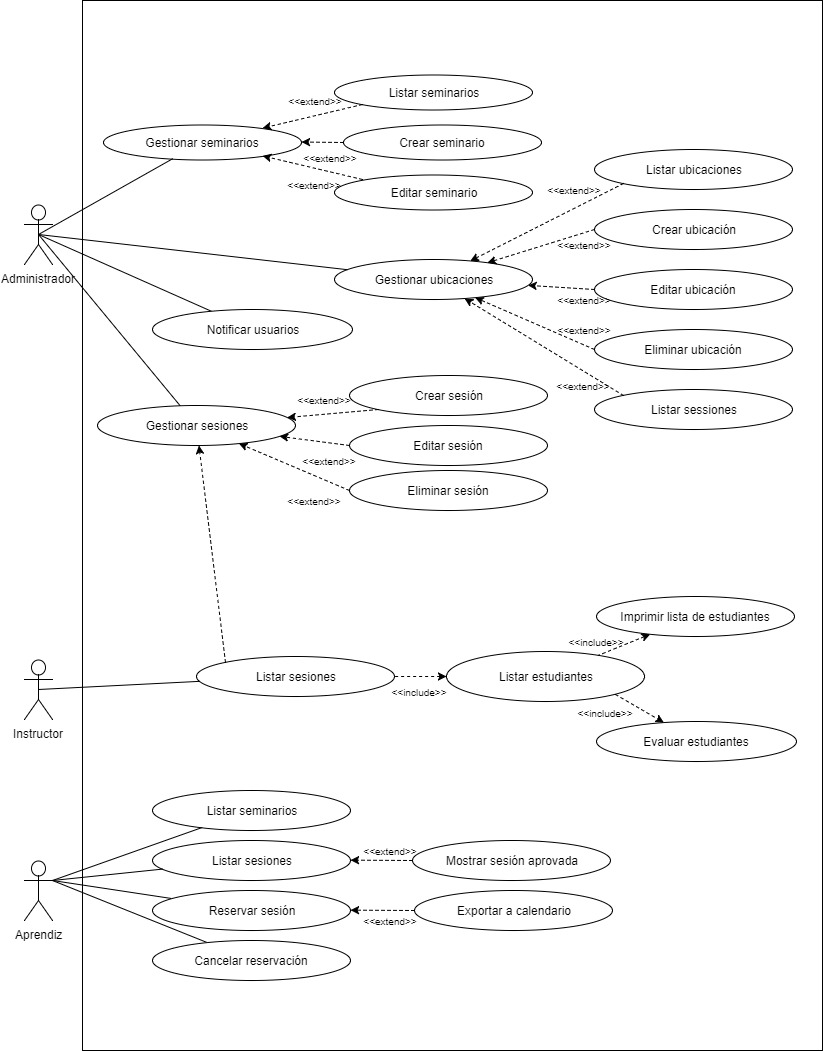
\includegraphics[width=0.77\textwidth]{figuras/diagramaCasosDeUso.jpg}
		\caption{Diagrama de casos de uso.} \label{fig:diagramaCasosDeUso}
	\end{center}
\end{figure}

\begin{figure}[t]
	\begin{center}
		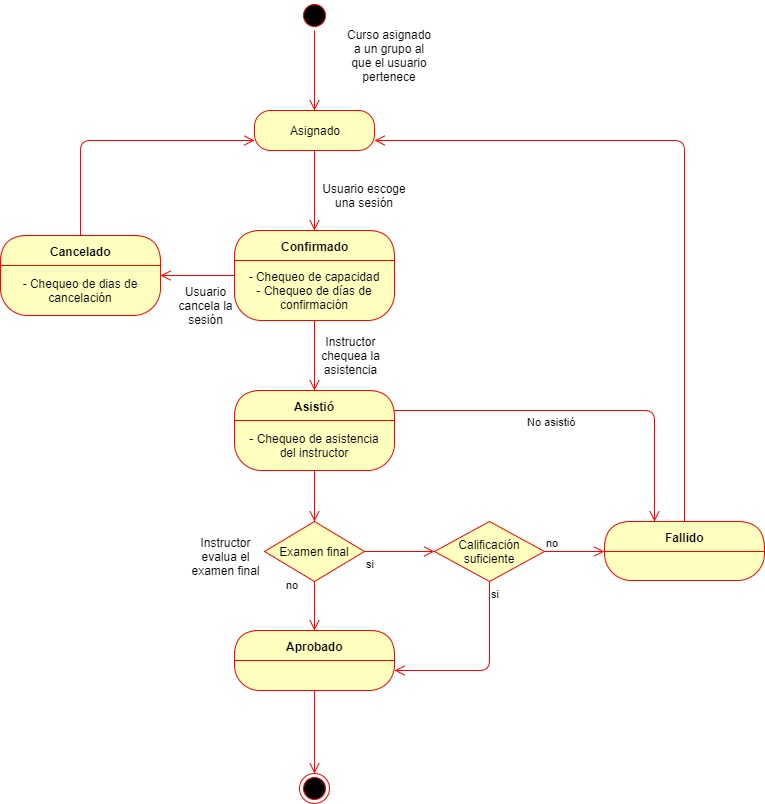
\includegraphics[width=\textwidth]{figuras/diagramaEstadosSesion.jpg}
		\caption{Diagrama que demuestra los distintos estados en los que se puede encontrar una sesión prensencial.} \label{fig:diagramaEstadosSesion}
	\end{center}
\end{figure}

\begin{figure}[t]
	\begin{center}
		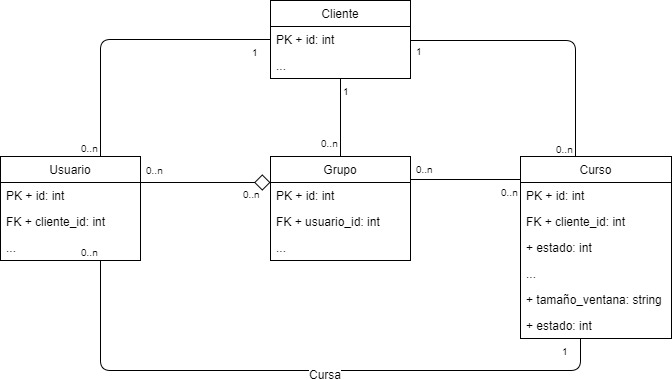
\includegraphics[width=0.9\textwidth]{figuras/databasePrevia.jpg}
		\caption{Diagrama UML parcial de la base de datos del SGA de FKC previa al proyecto.} \label{fig:baseDeDatosPrevia}
	\end{center}
\end{figure}

\begin{figure}[t]
	\begin{center}
		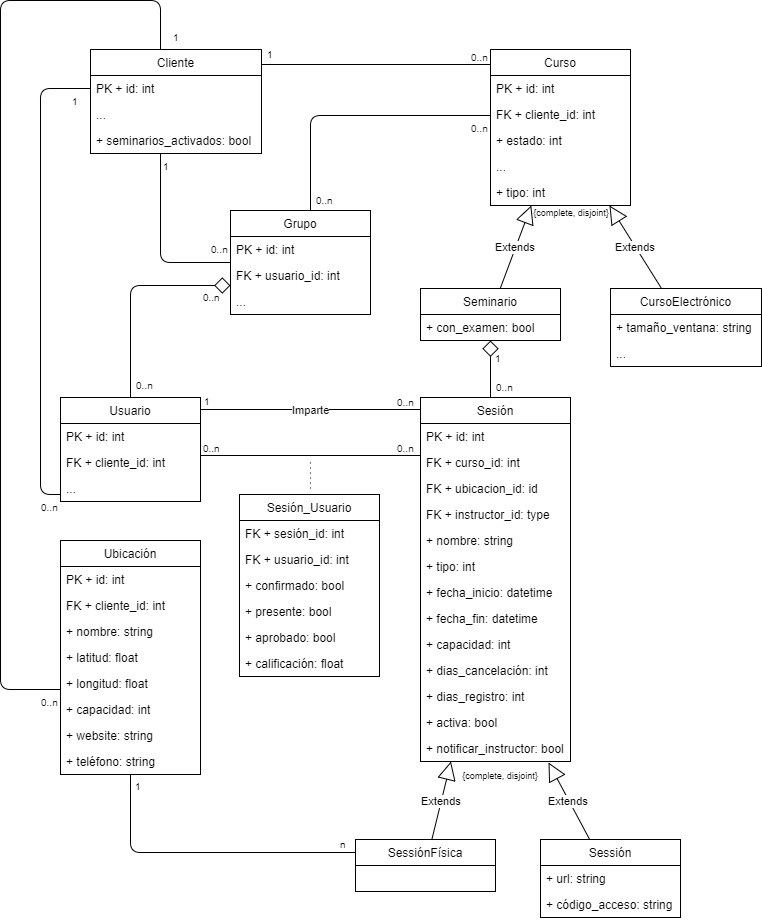
\includegraphics[width=\textwidth]{figuras/database.jpg}
		\caption{Diagrama UML parcial de la base de datos final del SGA de FKC.} \label{fig:baseDeDatosFinal}
	\end{center}
\end{figure}

\begin{figure}[t]
	\begin{center}
		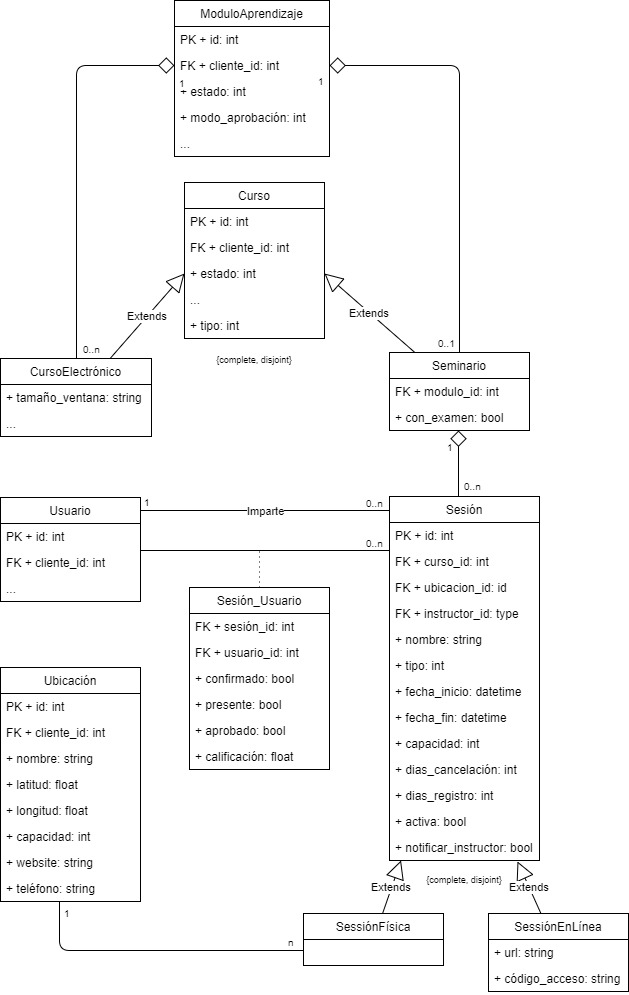
\includegraphics[width=0.8\textwidth]{figuras/databaseBibliomed.jpg}
		\caption{Diagrama UML parcial de la base de datos final del SGA de Bibliomed.} \label{fig:baseDeDatosBibliomed}
	\end{center}
\end{figure}

%%%%%%%%%%%%%%%%%%%%%%%%%%%%%%%%%%%%%%%%%%%%%%%%%%%%%%%%%%%%%%%%%%%%%%%%%%%%%%%%%%%%%%%%%%%%%
%%%%%%%%%%%%%%%%%%%%%%%%%%%%%%%        Screenshots            %%%%%%%%%%%%%%%%%%%%%%%%%%%%%%%
%%%%%%%%%%%%%%%%%%%%%%%%%%%%%%%%%%%%%%%%%%%%%%%%%%%%%%%%%%%%%%%%%%%%%%%%%%%%%%%%%%%%%%%%%%%%%

\chapter{Screenshots de los sistemas}


\begin{figure}[h]
	\begin{center}
		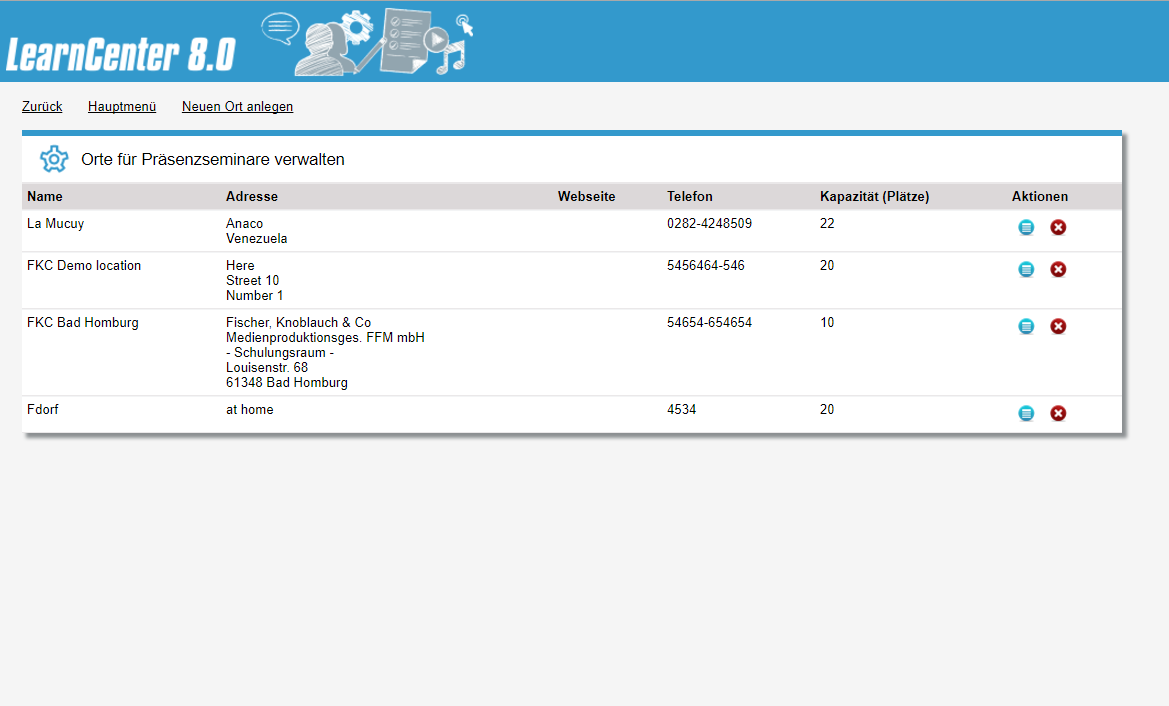
\includegraphics[width=\textwidth]{screenshots/listar_ubicaciones.png}
		\caption{Vista del listado de Ubicaciones.} \label{fig:listarUbicaciones}
	\end{center}
\end{figure}

\begin{figure}[h]
	\begin{center}
		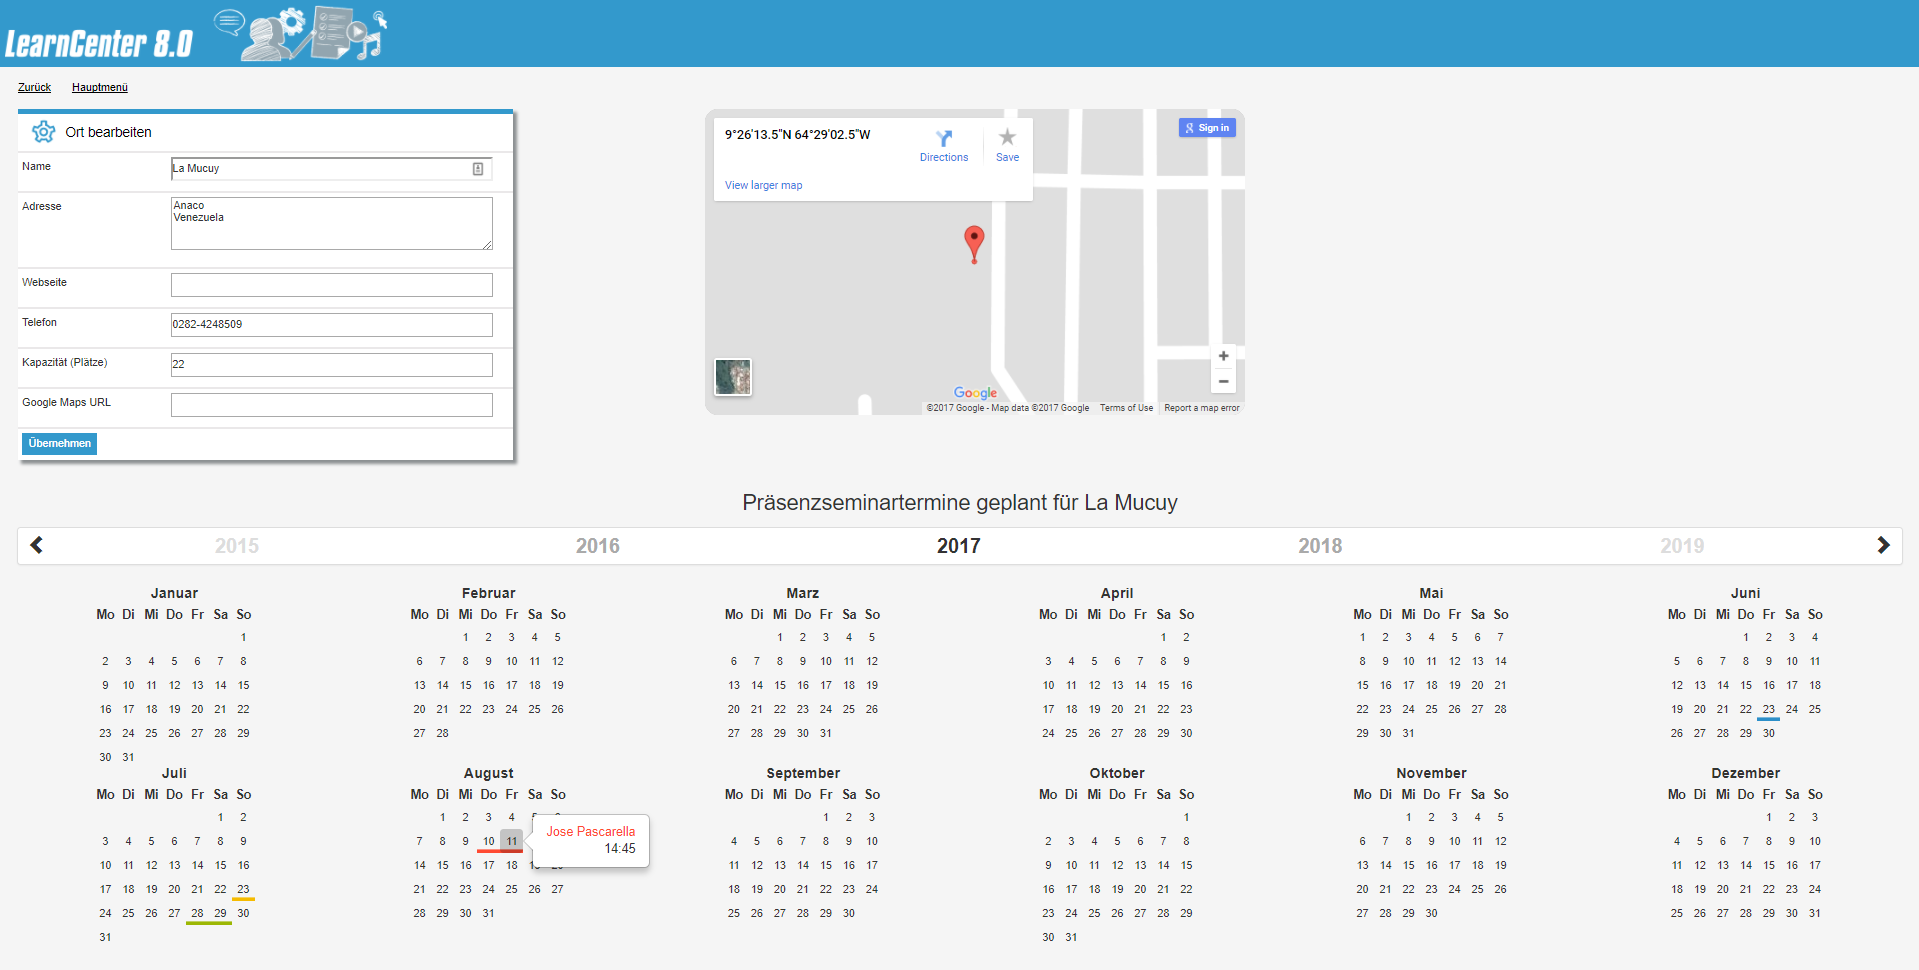
\includegraphics[width=\textwidth]{screenshots/edicion_ubicacion.png}
		\caption{Vista de la edición de una ubicación.} \label{fig:editarUbicaciones}
	\end{center}
\end{figure}

\begin{figure}[h]
	\begin{center}
		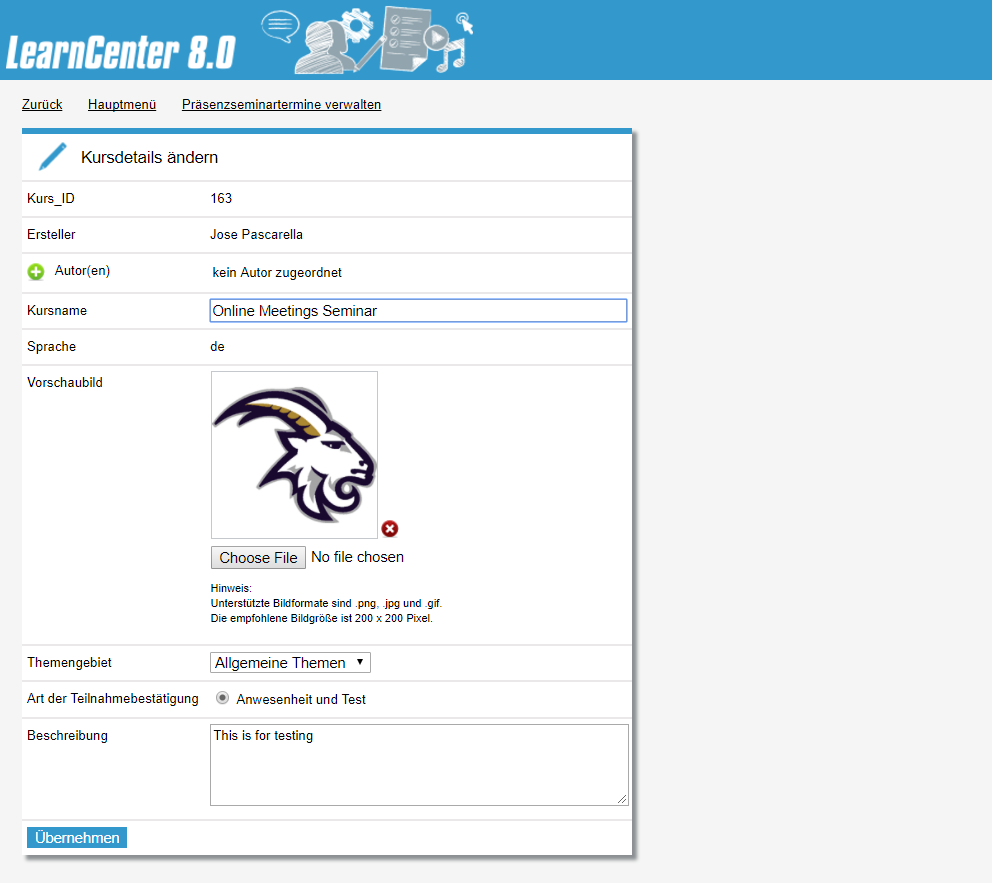
\includegraphics[width=\textwidth]{screenshots/creacion_seminario.png}
		\caption{Vista de la creación de un seminario.} \label{fig:creacionSeminario}
	\end{center}
\end{figure}

\begin{figure}[h]
	\begin{center}
		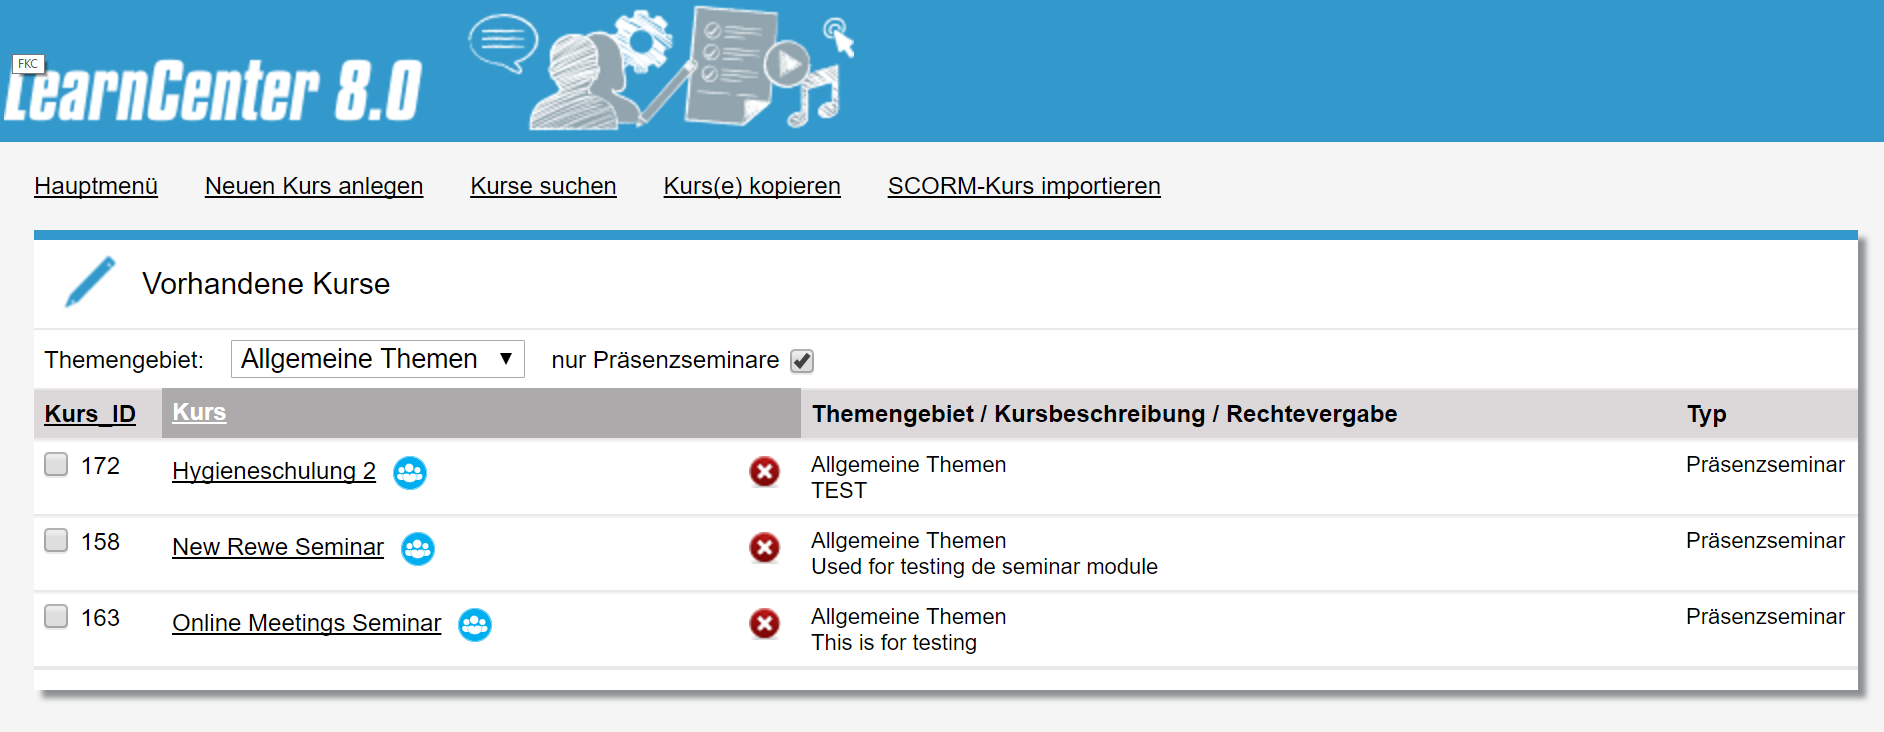
\includegraphics[width=\textwidth]{screenshots/admin_listar_cursos.png}
		\caption{Vista del listado de cursos del sistema para el administrador.} \label{fig:listarCursos}
	\end{center}
\end{figure}

\begin{figure}[h]
	\begin{center}
		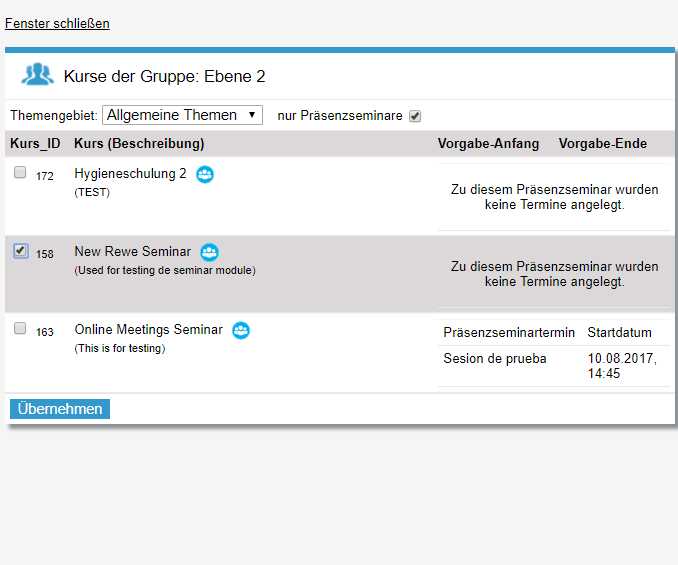
\includegraphics[width=\textwidth]{screenshots/asignar_seminario.png}
		\caption{Vista de la asignación de un seminario a un grupo.} \label{fig:asignarSeminario}
	\end{center}
\end{figure}

\begin{figure}[h]
	\begin{center}
		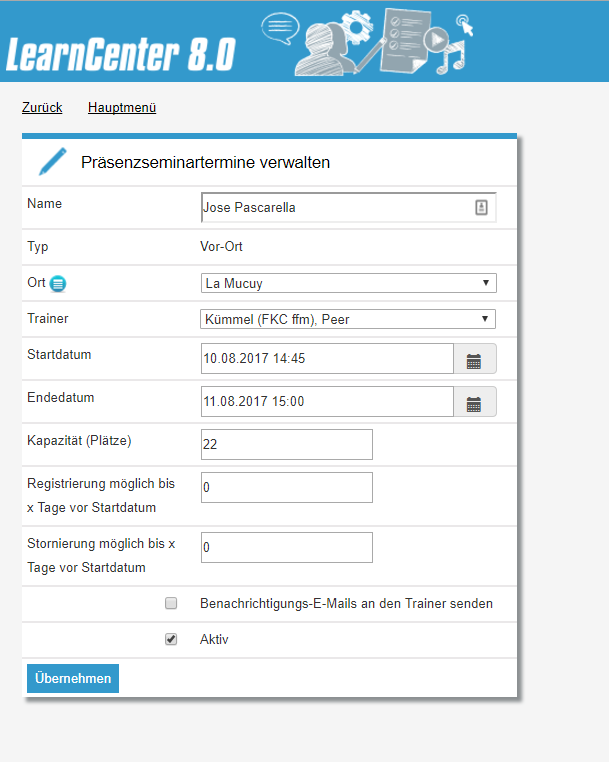
\includegraphics[width=\textwidth]{screenshots/creacion_seminario_sesion.png}
		\caption{Vista de la creación de una sesión de un seminario.} \label{fig:creacionSesion}
	\end{center}
\end{figure}

\begin{figure}[h]
	\begin{center}
		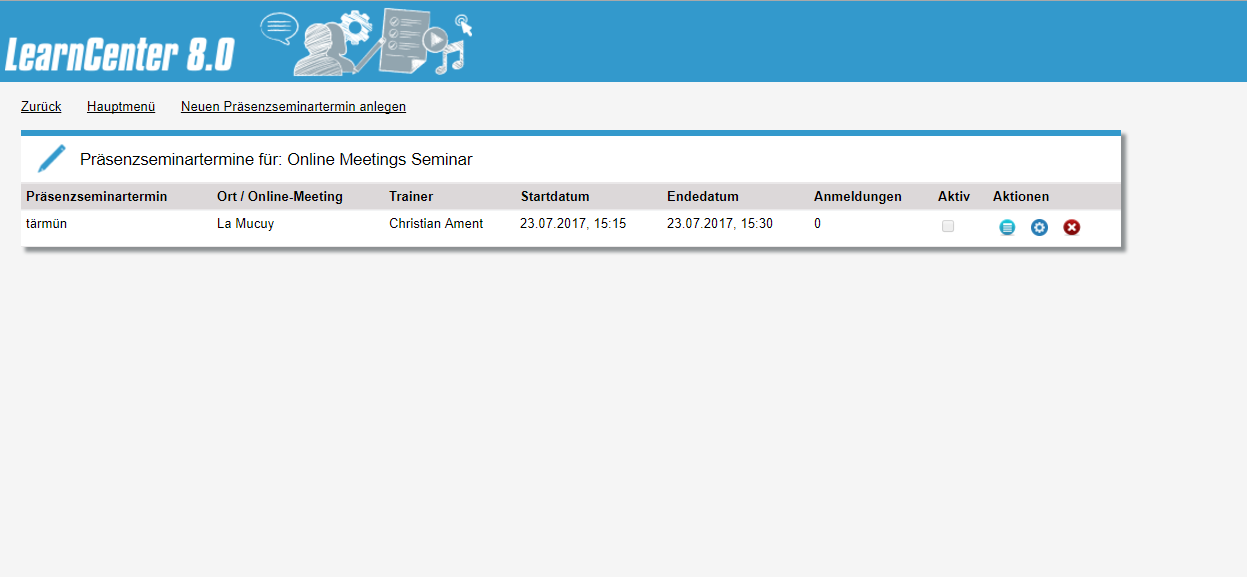
\includegraphics[width=\textwidth]{screenshots/listar_sesiones_seminario.png}
		\caption{Vista del listado de las sesiones de un seminario.} \label{fig:listarSesiones}
	\end{center}
\end{figure}

\begin{figure}[h]
	\begin{center}
		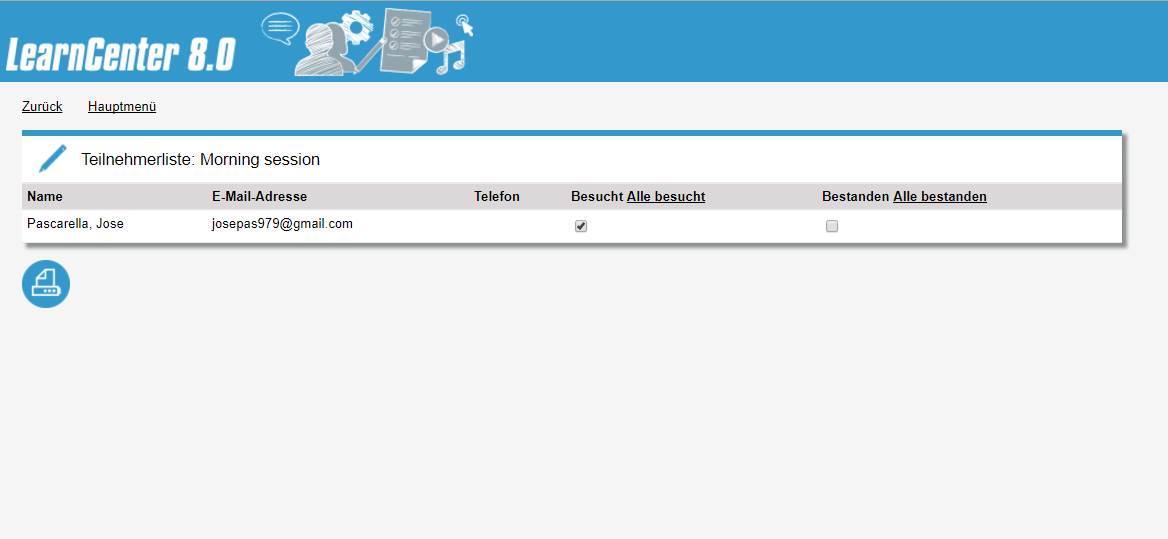
\includegraphics[width=\textwidth]{screenshots/manage_session.png}
		\caption{Vista de los cursos de un instructor.} \label{fig:gestionarSesion}
	\end{center}
\end{figure}

\begin{figure}[h]
	\begin{center}
		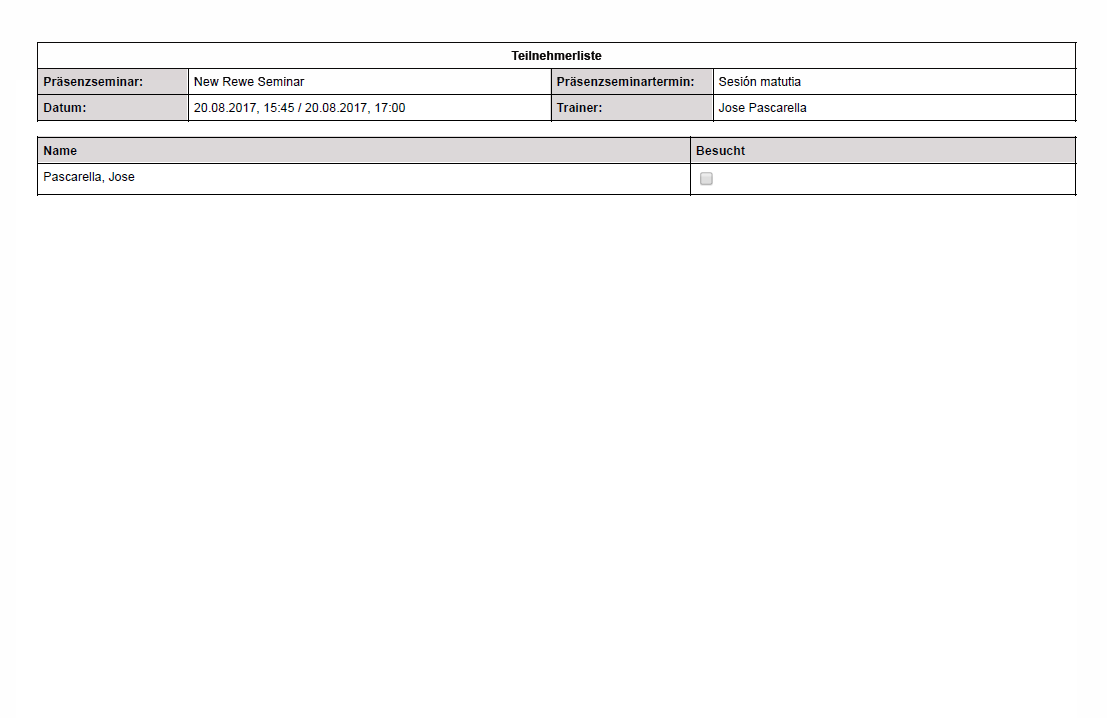
\includegraphics[width=\textwidth]{screenshots/lista_alumnos.png}
		\caption{Archivo PDF generado con la lista de los estudiantes de un curso.} \label{fig:listarAlumnos}
	\end{center}
\end{figure}

\begin{figure}[h]
	\begin{center}
		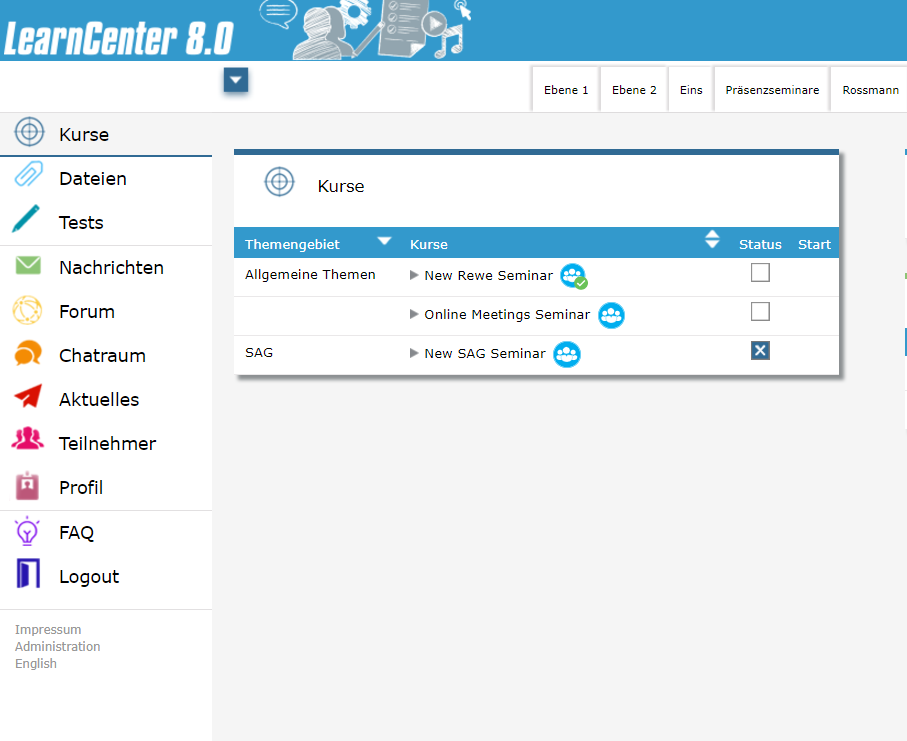
\includegraphics[width=\textwidth]{screenshots/user_listar_cursos2.png}
		\caption{Vista de los cursos disponibles para el usuario aprendiz.} \label{fig:aprendizListarCursos}
	\end{center}
\end{figure}

\begin{figure}[h]
	\begin{center}
		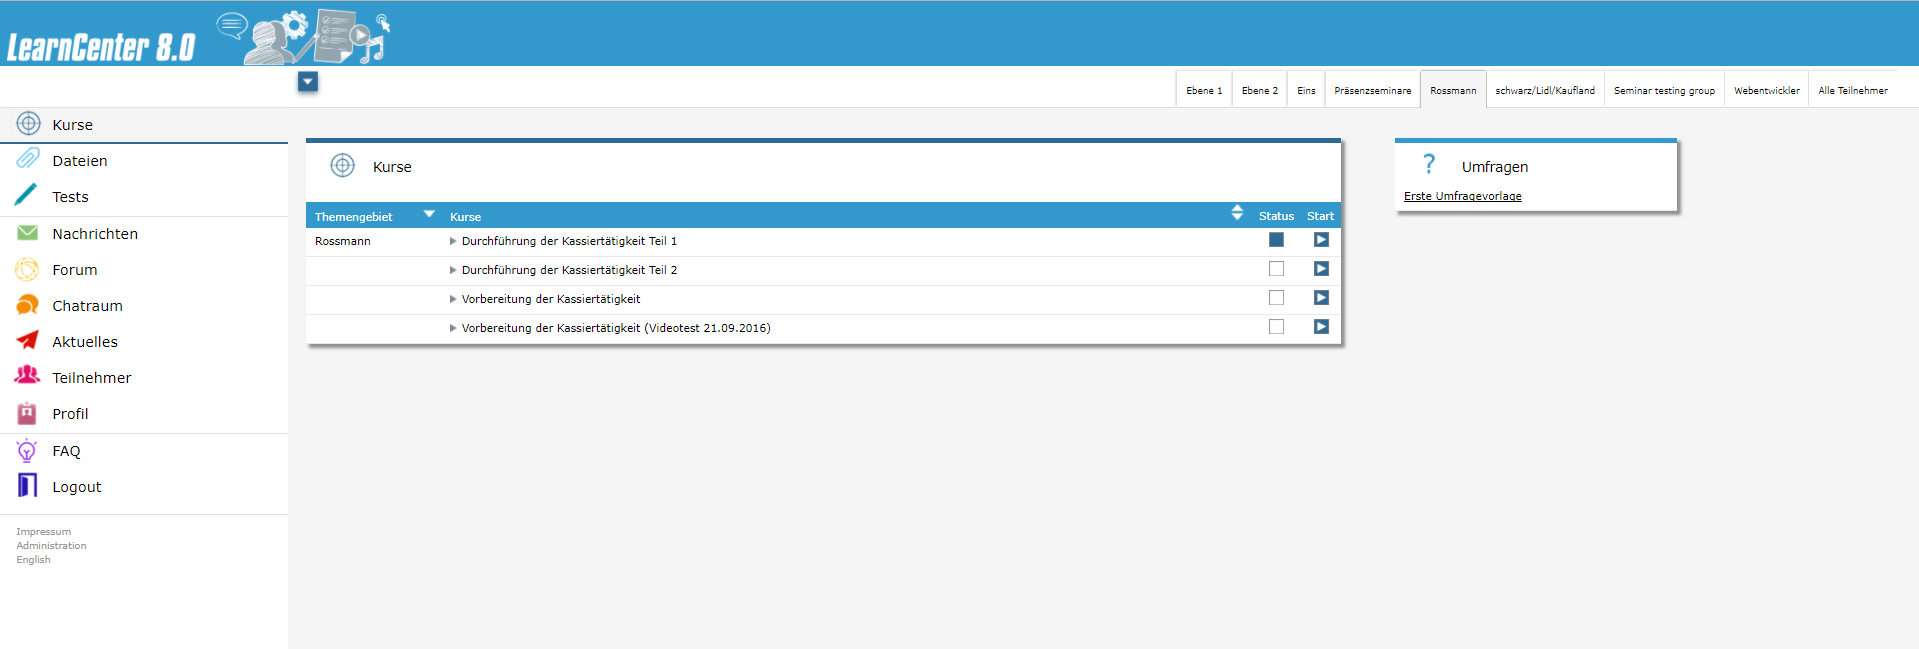
\includegraphics[width=\textwidth]{screenshots/user_listar_seminar_viejo.png}
		\caption{Vista de los cursos disponibles para el usuario aprendiz antes de la extensión realizada en la pasantia.} \label{fig:aprendizListarViejo}
	\end{center}
\end{figure}

\begin{figure}[h]
	\begin{center}
		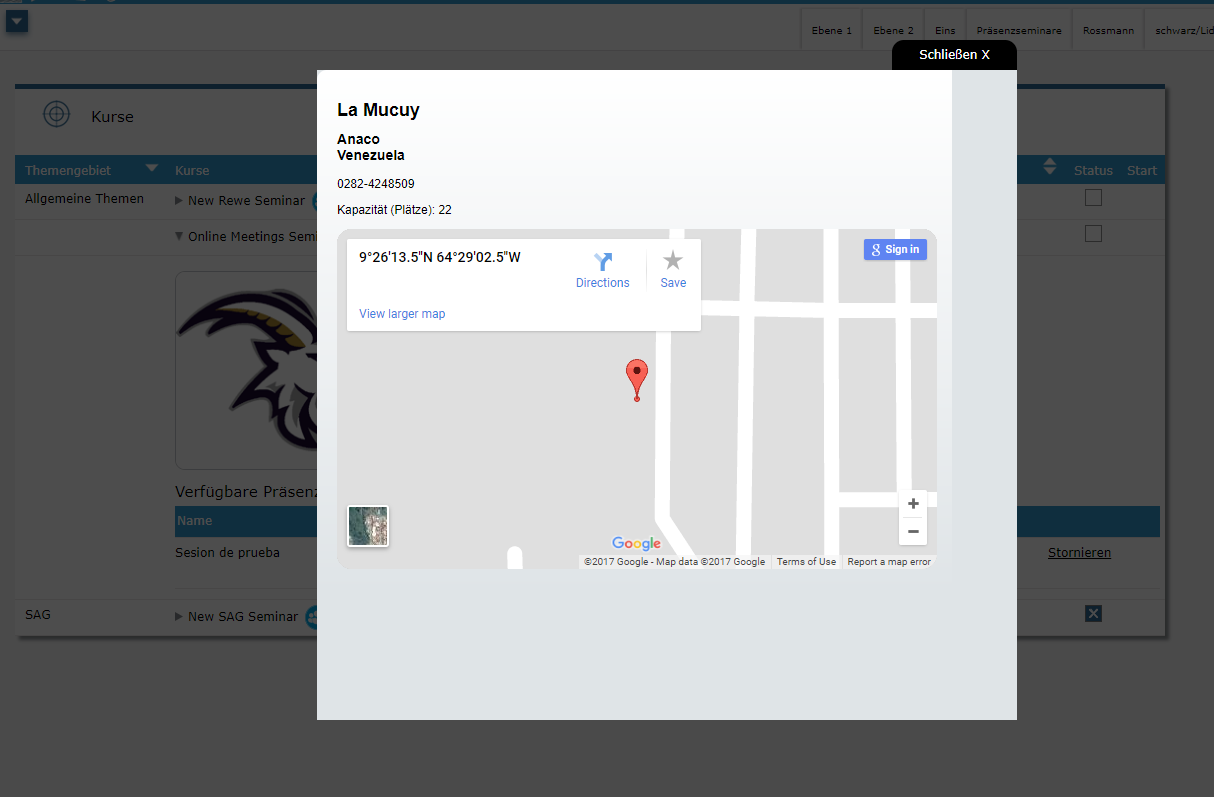
\includegraphics[width=\textwidth]{screenshots/modal_ubicacion.png}
		\caption{Vista del modal mostrado con los datos de la ubicación de la sesión correspondiente.} \label{fig:modalUbicacion}
	\end{center}
\end{figure}

\begin{figure}[h]
	\begin{center}
		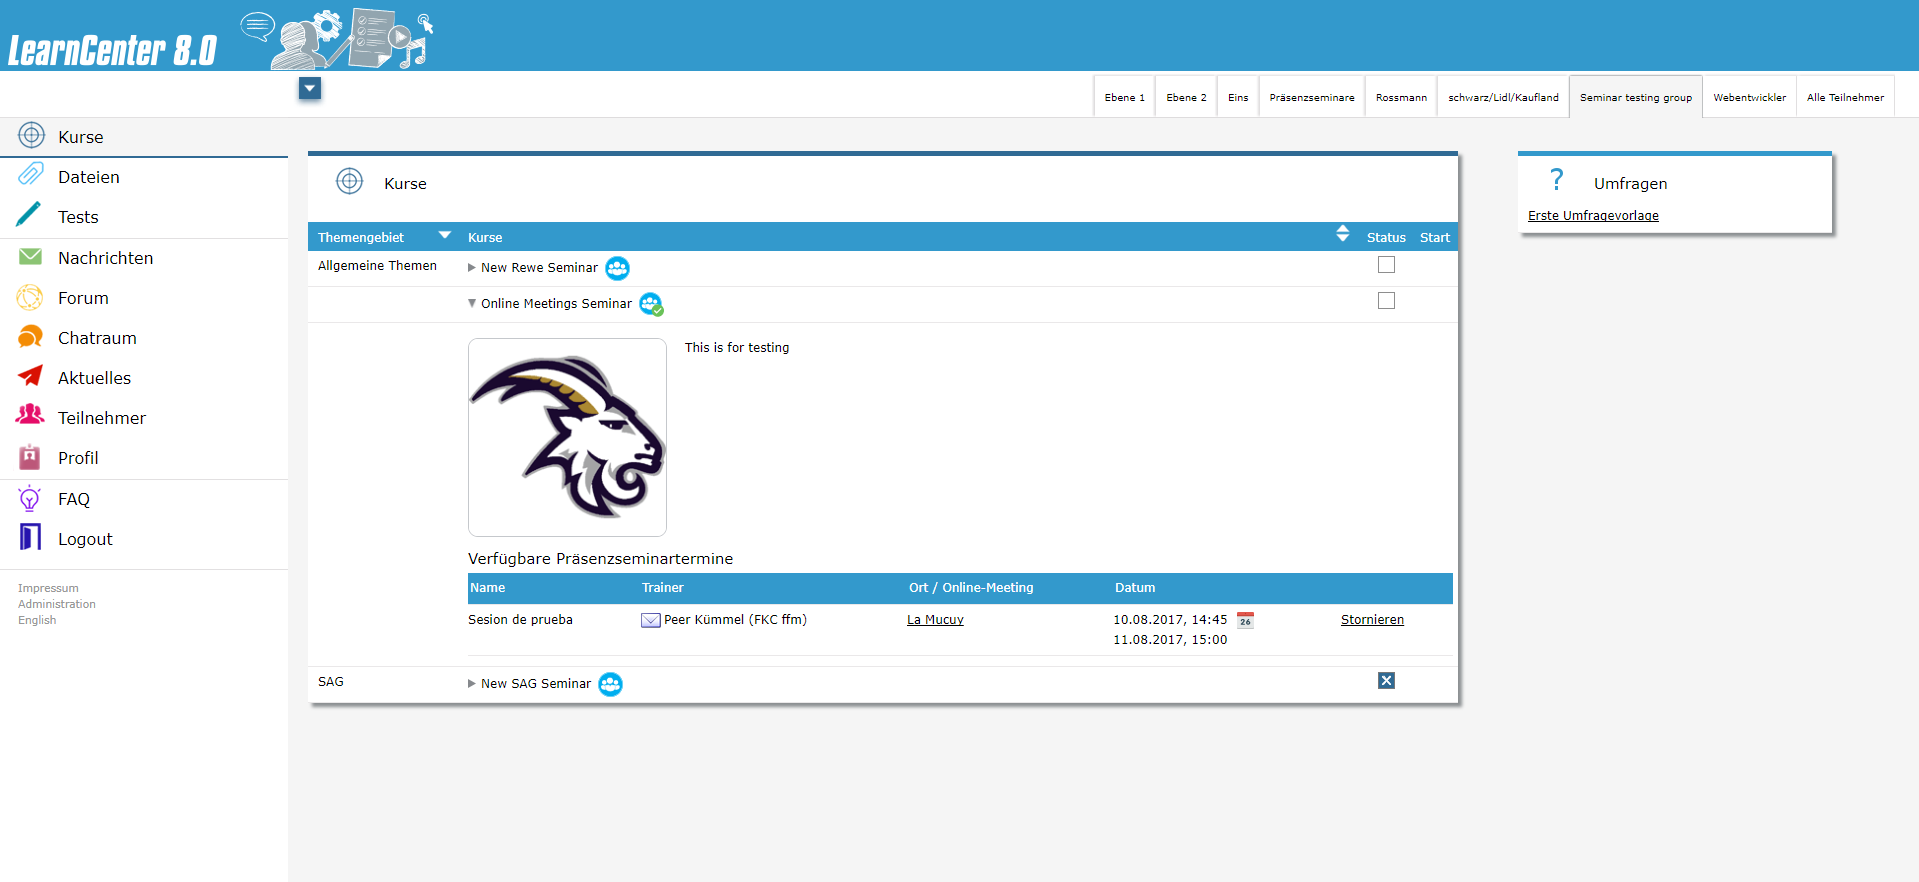
\includegraphics[width=\textwidth]{screenshots/user_reservar.png}
		\caption{Vista de una sesión confirmada por el usario.} \label{fig:usuarioSesionConfirmada}
	\end{center}
\end{figure}

\begin{figure}[h]
	\begin{center}
		
\includegraphics[width=\textwidth]{screenshots/emails.png}
		\caption{Formato de los correos enviados por el sistema.} \label{fig:correos}
	\end{center}
\end{figure}

\begin{figure}[h]
	\begin{center}
		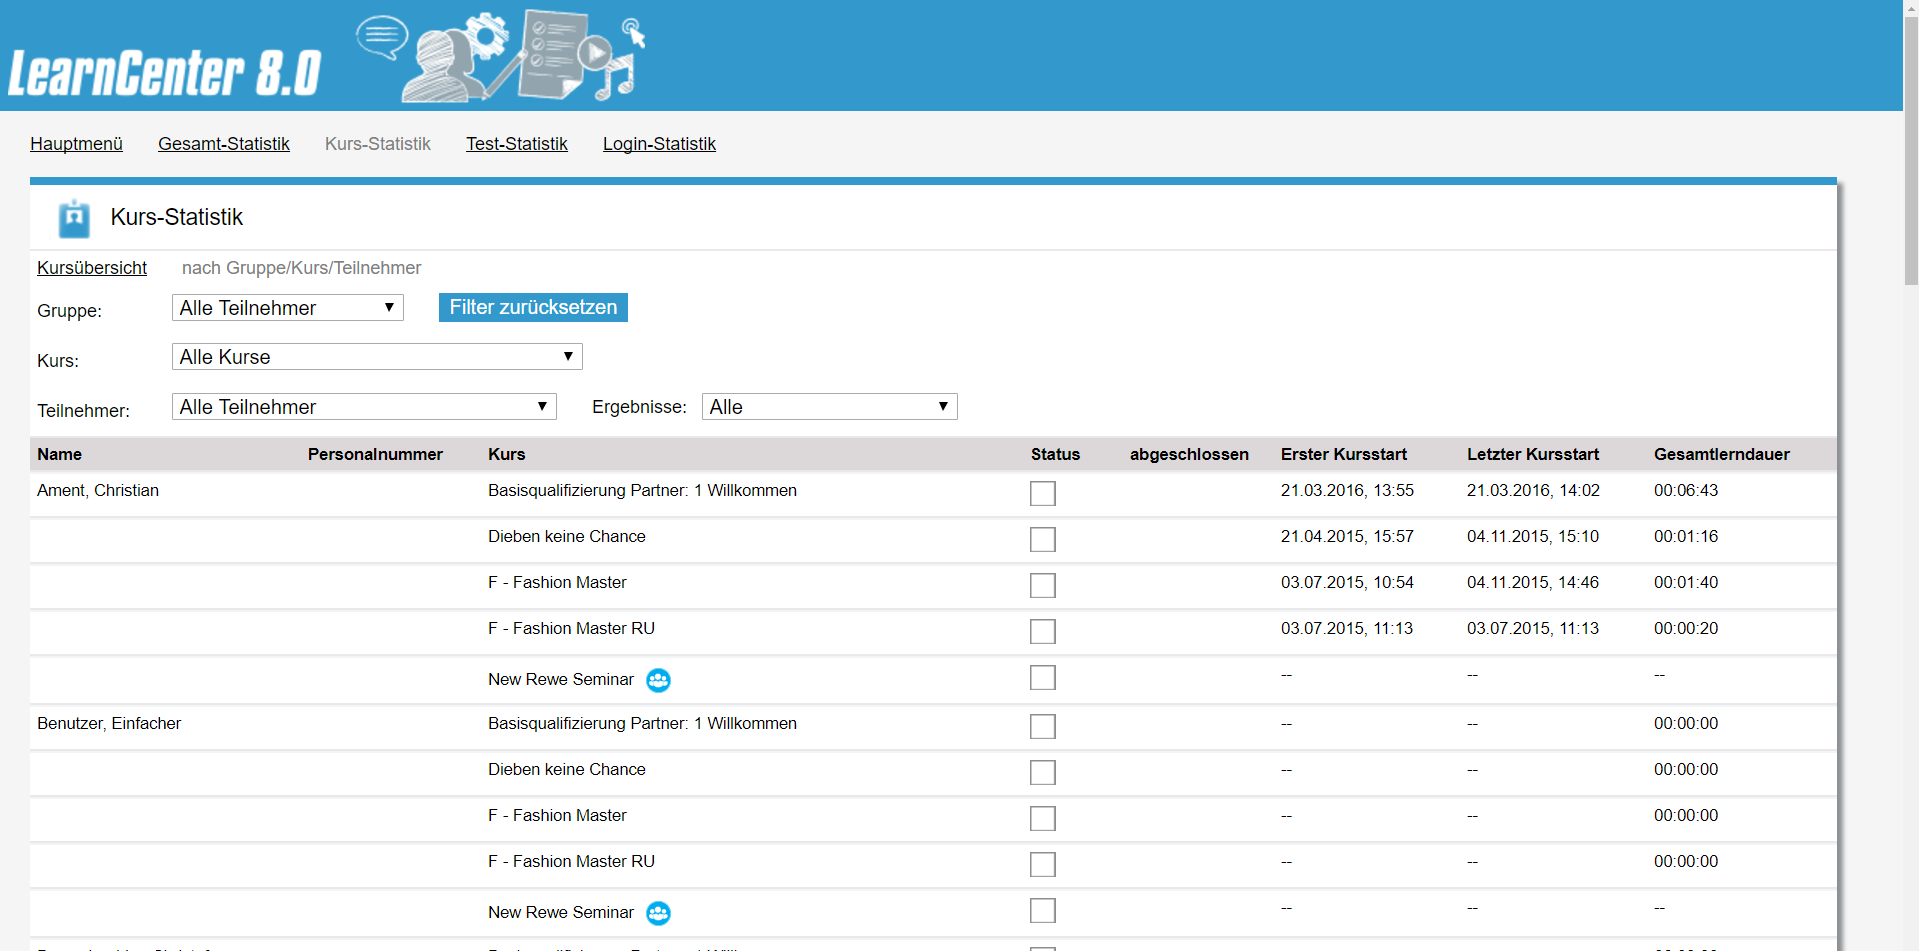
\includegraphics[width=\textwidth]{screenshots/estadisticas.png}
		\caption{Vista de las estadísticas mostradas al administrador.} \label{fig:estadisticasAdmin}
	\end{center}
\end{figure}

\begin{figure}[h]
	\begin{center}
		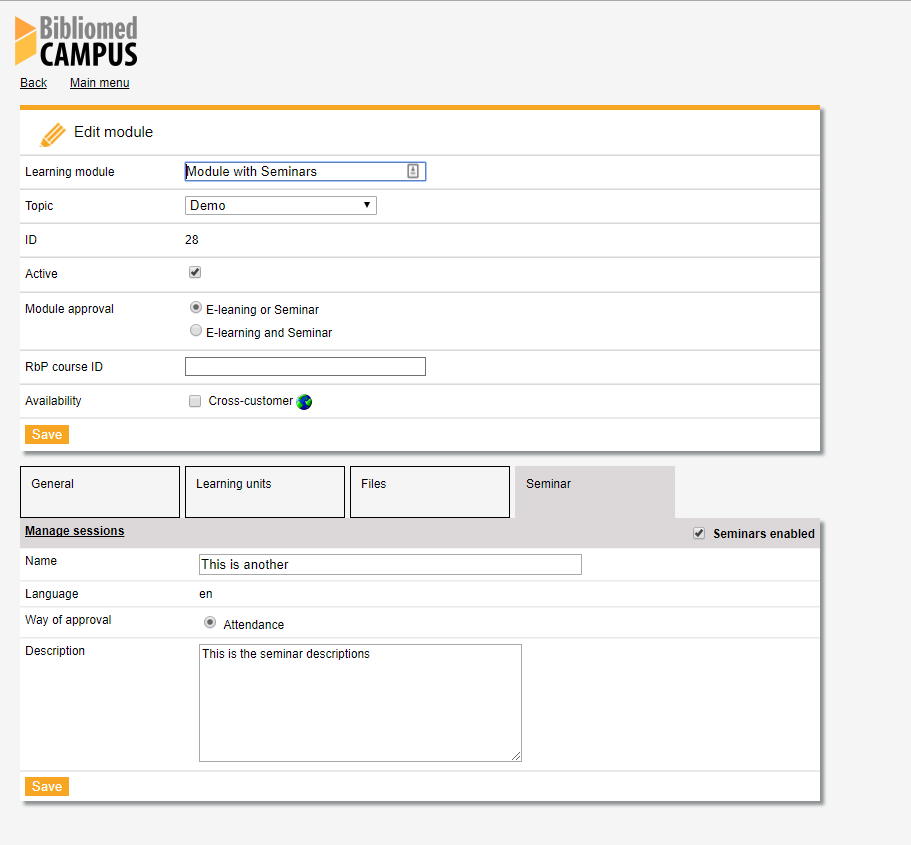
\includegraphics[width=\textwidth]{screenshots/bibliomed_adaptacion.png}
		\caption{Vista de la adaptación hecha para la creación de seminarios en el SGA de Bibliomed.} \label{fig:creacionSeminarioBibliomed}
	\end{center}
\end{figure}

\begin{figure}[h]
	\begin{center}
		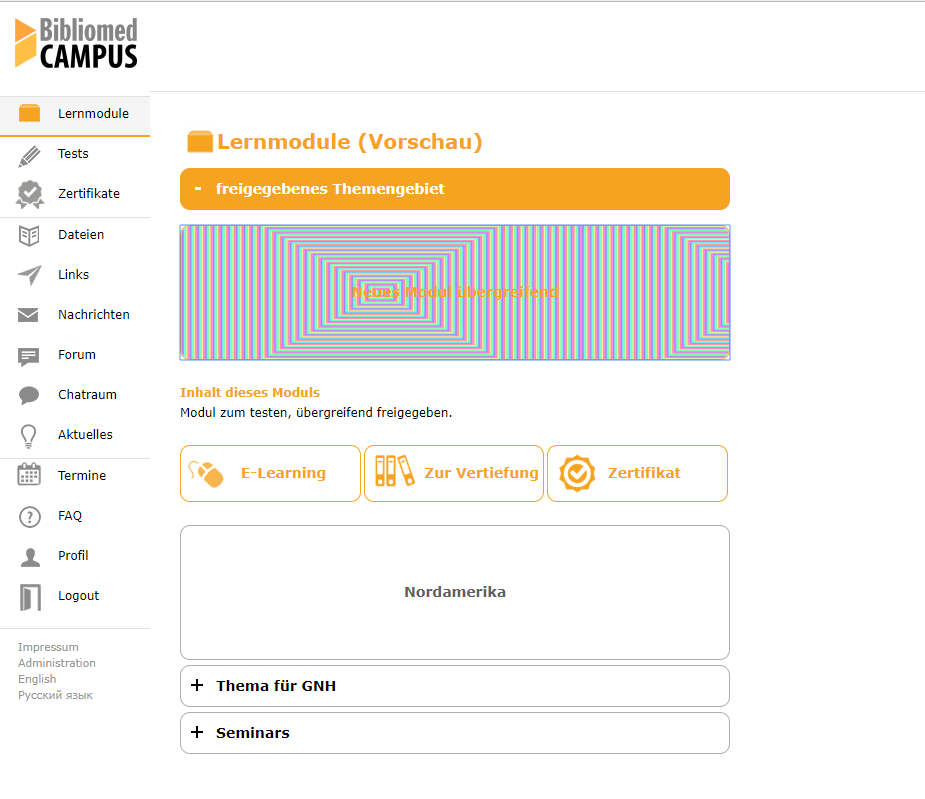
\includegraphics[width=\textwidth]{screenshots/bibliomed_viejo.png}
		\caption{Vista de cursos disponibles para el aprendiz antes de la integración de el módulo de seminarios en el SGA de Bibliomed.} \label{fig:bibliomedViejo}
	\end{center}
\end{figure}

\begin{figure}[h]
	\begin{center}
		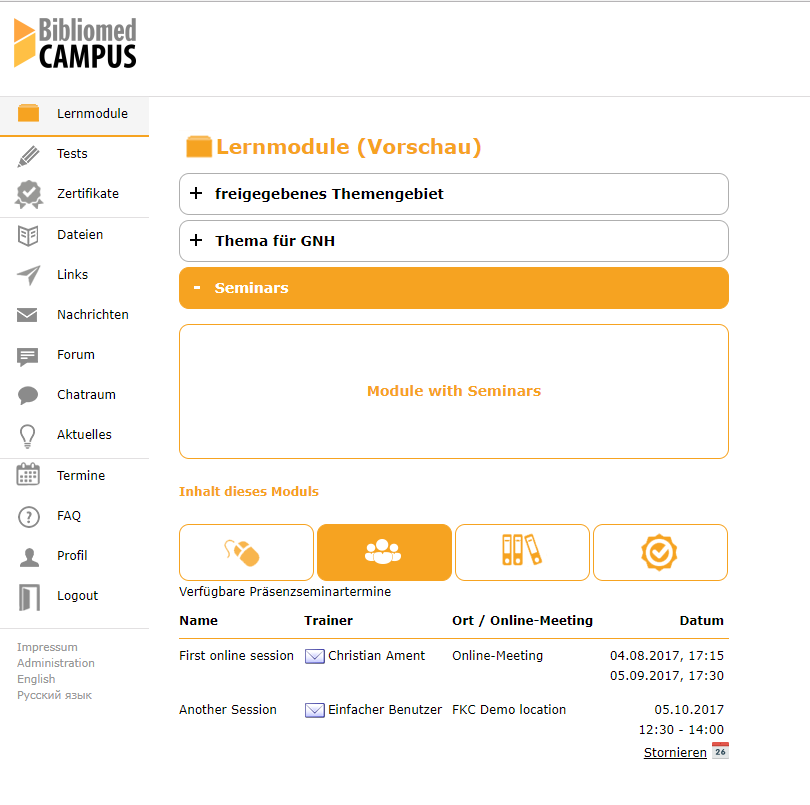
\includegraphics[width=\textwidth]{screenshots/bibliomed_reservar_sesion.png}
		\caption{Vista de una sesión reservada en el SGA de Bibliomed.} \label{fig:reservarSesiónBiliomed}
	\end{center}
\end{figure}















\end{document}